\chapter{Results}
\label{ch:res}

In this chapter we explain how we use the forward model to generate data and how we set up a Bayesian framework to then give distribution of solutions.
Here we make it explicit and proivde all information to be able to replciate our results.
In this work we simulate datawith an ozone profile from \cite{}.
We follow the U.S. standard atmosphere, 1976 \cite{} to relate pressure and temperature and hieght and the HITRANonline \cite{} database to calculate the measured signal.\expandafter\string\the\font 
We follow the mipas instrument description fro the froward model \cite{}.

\section{Simulate Data}
Ground truth
We take an ozone profile generated from some MLS Data \cite{MLSdata} in the Antarctic region.
This gives us pressure values and Ozone volume mixing ratio values.
We connect pressure and height values with the hydrostatic equilibrium equation
\begin{align}
	\frac{\text{d}p}{p} = \frac{- g M}{R^* T} \text{d} h \, ,
\end{align}
which holds up to a geometric height of $84.356$km, which is also the the boarer of the atmospher we set.
\begin{align}
	g = g_0 \Bigg( \frac{r_0}{r_0 + h} \Bigg) \, ,
\end{align}
with $r_0 \approx 6356 \, \text{km}$ (also known as the polar radius of the earth) and $g_0 \approx 9.81 \text{m}/\text{s}^2$ and \cite{}.
with the universal gas consant $R^* \approx 8.314  \, \text{N m} / \text{mol} / \text{K}$. The molecules number ... is $M = M_0 \approx 28.97 \, \text{kg}/\text{mol}$ for altiudes below 79km \cite{}.
We ignore the difference of $.0004\%$

We take Temparute values 
\begin{align}
	T(h) = \begin{cases*}
		T_0, & \text{$h = 0$}\\
		T_0 + a_0 h , & \text{$0 \leq h < h_{1}$}\\
		T_0 + a_0 h_{1}, & \text{$h_{1} \leq  h < h_{2}$}\\
		T_0 + a_0 h_{1} + a_1 (h   - h_2),  & \text{$h_{2} \leq h < h_{3}$}\\
		T_0 + a_0 h_{1} + a_1 (h_{3} - h_{2}) + a_2 (h   - h_3), & \text{$h_{3} \leq h < h_{4}$}\\
		T_0 + a_0 h_{1} + a_1 (h_{3} - h_{2}) + a_2 (h_{4} - h_{3}), & \text{$h_{4} \leq h < h_{5}$}\\
		T_0 + a_0 h_{1} + a_1 (h_{3} - h_{2}) + a_2 (h_{4} - h_{3}) + a_3 (h   - h_{5}), & \text{$h_{5} \leq h < h_{6}$}\\
		T_0 + a_0 h_{1} + a_1 (h_{3} - h_{2}) + a_2 (h_{4} - h_{3}) + a_3 (h_{6} - h_{T5}) + a_4 (h - h_{6}), & \text{$h_{6} \leq h \lesssim 85$}
	\end{cases*} 
	\label{eq:tempFunc}
\end{align}
from the \cite{atmosphere1976us},We can formulate a temperature function from \cite{atmosphere1976us}
where the geometric height height values are
$h_{1} = 11$km
$h_{2} = 20.1$km
$h_{3} = 32.2$km
$h_{4} = 47.4$km
$h_{5} = 51.4$km
$h_{6} = 71.8$km
$a_{0} = -6.5$K/km
$a_{1} = 1$K/km
$a_{2} = 2.8$K/km
$a_{3} = -2.8$K/km
$a_{4} = -2$K/km
depending on 12 parameters with values provided by \cite{}, also see table \ref{}.
We set this as our true temperature profile and refer to \cite{} for temperature values above $79 \,\text{km}$.


\cite{CubeSatInternal}
\cite{MLSdata}
\cite{vsimevckova2006einstein}
\cite{christentwalkaccess}
\cite{Fox_ISBA2008}
\cite{mipas2000handbook}
\cite{gordon2022hitran2020}
\cite{atmosphere1976us}



Then we can calculate data vector with a pointing accuracy $0.0075$ which is equal ot arc as request by \cite{CubeSatInternal}.
Then we get $m = $ in between an atmosphere of $h_{L,0} = $ and $h_{L,n} = $, where the layers are dictated by the MLS data.
at wave number $\nu = $ where ozone is most dominant
According to Equation
With voltage SNR = $60$.

Given the calculte pressure value we can fit an exponentila within the rehion our interest the atmospheric layers

The pressure function,
\begin{align}
	p(h) =
	\exp{ \{ -b \,  (h - h_{0} ) \} } \,  p_0 \, ,
	\label{eq:pressFunc}
\end{align}
is depending on three different parameters, the gradient $b$ and the tuple $(p_0,h_{0})$.

Where the ground truth values for that are 

\section{Set up Bayesian model}
\begin{itemize}
	\item fill in what we descrube beofre 
	\item describe parametres and hyper paraemrets set up model to make dag
	\item then prior modelling
\end{itemize}
In this section we present the explicit Bayesian we will use to recover pressure temperature and ozone values.
On big parts of bayesina modeling is prior modelling where we set up the model
figure out correltaion with DAG
and choose priors as uninformtivae as we can 
and accordfing to physical propoeritesd if we can 
\subsection{DAG}
Again we draw a DAG and specify prior disribtoin over those

\begin{itemize}
	\item correlation structure between ozone and temperature and pressure
\end{itemize}
\begin{figure}[thb!]
	\centering
	\begin{tikzpicture}
		\node[roundnode2] at (-4.5,6.5) (Q)     {$\bm{Q}$};
		\node[roundnode2] at (-3,5) (x)     {$\bm{x}$};
		\node[align=center] at (-1,4) (A)    {$\bm{A}(\bm{x},\bm{p},\bm{T})$};
		\node[roundnode2] at (-1,2.5) (u)    {$\bm{\Omega}$};
		\node[rectnode] at (-1,1) (y)    {$\bm{y}$};
		\node[roundnode2] at (-2.5,2.5) (e)    {$\bm{\eta}$};
		\node[roundnode2] at (-6.25,6.5) (S)    {$\bm{\Sigma}$};
		\node[roundnode2] at (-7.75,8) (s)    {$\gamma$};
		\node[roundnode2] at (-6,8) (d)    {$\delta$};
		\node[roundnode2] at (3,6.5) (t)     {$\bm{T}$};
		\node[roundnode2] at (-1,6.5) (p)     {$\bm{p}$};
		\node[roundnode2] at (1,5) (pt)     {$\bm{p}/\bm{T}$};
		\node[roundnode2] at (0,8) (b1)    {$b$};
		%\node[roundnode2] at (1,8) (b2)    {$b_2$};
		\node[roundnode2] at (-2,8) (h1)    {$h_{0}$};
		\node[roundnode2] at (-1,8) (p0)    {$p_0$};
		\node[roundnode2] at (2.25,8) (ht)    {$\bm{h}_T$};
		\node[roundnode2] at (3.25,8) (ct)    {$T_0$};
		\node[roundnode2] at (4.25,8) (at)    {$\bm{a}$};
		
		%Lines
		\draw[->, very thick] (S.south east) -- (e.north west);
		\draw[->, mydotted, very thick] (s.south east) -- (S.north west);
		\draw[->, very thick] (u.south) -- (y.north);
		\draw[->, mydotted, very thick] (A.south) -- (u.north);
		\draw[->, mydotted,  very thick] (x.south east) -- (A.west);
		\draw[->, mydotted, very thick] (p.south east) -- (pt.north west);
		\draw[->, mydotted, very thick] (t.south west) -- (pt.north east);
		\draw[->, mydotted, very thick] (pt.south west) -- (A.east);
		\draw[->, mydotted, very thick] (h1.south) -- (p.north west);
		\draw[->, mydotted, very thick] (p0.south) -- (p.north);
		\draw[->, mydotted, very thick] (b1.south) -- (p.north east); 
		%\draw[->, very thick] (b2.south) -- (p.east); 
		\draw[->, mydotted, very thick] (d.south east) -- (Q.north west); 
		\draw[->, mydotted, very thick] (e.south east) -- (y.west); 
		
		\draw[->, very thick] (Q.south east) -- (x.north west); 
		\draw[->, mydotted, very thick] (ht.south) -- (t.north west);
		\draw[->, mydotted, very thick] (ct.south) -- (t.north);
		\draw[->, mydotted, very thick] (at.south) -- (t.north east);
		%\node[align=center] at (0.25,3.95) (f3) {$\approx \bm{M A}_L$};
	\end{tikzpicture} 
\caption[Complete directed acyclic graph of the forward model.]{Complete directed acyclic graph of the forward model. The hyper-parameters at the top deterministically (dotted line) describe the parameters ($\bm{p}/\bm{T}$) or the noise covariance $\bm{\Sigma} = \gamma^{-1} \bm{I}$ of the random (solid line) noise $\bm{\eta} \sim \mathcal{N}(0,\gamma^{-1} \bm{I} ) $ and precision matrix $\bm{Q} = \delta \bm{L}$ of the distribution of $\bm{x}\sim \mathcal{N}(0,\delta \bm{L}) $, where $\bm{L}$ is a graph Laplacian as in Eq. \ref{eq:GLapl}. We can group the noise precision $\gamma$  and the smoothness parameter $\delta$ to define the marginal posterior over those hyper-parameters and then condition on them for the conditional posterior distribution,for further details see Fig. \ref{fig:DAGO3}. In this whole process where we condition on the pressure $\bm{p}$ and temperature $\bm{T}$, which we retrieve separately, see Fig. \ref{fig:DAGPT}. The hyper-parameters $h_0,p_0,b$ deterministically describe the pressure function in Eq. \ref{eq:pressFunc}, note that we only need three parameters here since $h_0< h_{L,0}$ and $\bm{h}= \{ h_1, h_2,h_3,h_4,h_5,h_6\}$, $\bm{a} = \{ a_0, a_1, a_2,a_3,a_4\}$ and $T_0$ determine the temperature function.
The parameters $\bm{x}$ and $\bm{p}/ \bm{T}$ determine the space of all measurable noise free data $\bm{\Omega}$ through the forward model $\bm{A}(\bm{x},\bm{p},\bm{T})$ from which we randomly observe data set plus some random noise.}
\label{fig:DAGComplete}
\end{figure}

\subsection{Prior Modelling}
\begin{itemize}
	\item physical meaning by choosing priors
	\item eventuel depednices
	\item draw samples form priors should be as loose as possible
\end{itemize}
\begin{table}
	\centering
	\begin{tabular}{ |c||c|c|c|c|   }
		\hline
		& &\multicolumn{2}{|c|}{TT bounds}&\\
		\hline
		model parameters& priors&\makecell{lower}& \makecell{upper\\
		}&Context\\
		\hhline{|=||=|=|=|=|}
		$\gamma$ & $\mathcal{T}(1,10^{-10})$ &$5 \, 10^{-8}$ &$4.5 \, 10^{-7}$& $\bm{y}$\\ \hline
		$\delta$ &$\mathcal{T}(1,10^{-10})$ & -&-& $\bm{x}$\\ \hline
		$\lambda$ &- & 500&7000& $\bm{x}$\\ \hline
		$\bm{x}$ &$\mathcal{N}(0,\delta \bm{L})$ & -&-& $\bm{x}$\\ \hhline{|=||=|=|=|=|}
		%$\gamma$ & $\mathcal{N}(2.58e-9,2.58e-11)$ &2.45e-9&2.7e-9 &$\bm{x}$\\
		%$\delta_0$ &  $\mathcal{N}(0.8e-4,0.75e-5)$& 4e-5 & 1.1e-4&$\bm{x}$\\
		%$a_0$ &  $\mathcal{T}(3,1e6)$& 1e-15&1e-5&$\bm{x}$\\ \hline
		%$h_0$ &  $\mathcal{N}(31.35,1)$&27 &35&$\bm{x}$\\ \hline
		$h_0$ &  $\mathcal{N}(5.5,0.5)$& 4.76&5.74&$\bm{p/T}$\\ \hline
		$p_0$ &  $\mathcal{N}(500,6)$&479 &519&$\bm{p/T}$\\ \hline
		$b$ &  $\mathcal{N}(0.167,7\,10^{-4})$& 0.165& 0.170 &$\bm{p/T}$\\ \hline
		%$b_2$ & $\mathcal{N}(0.13,0.067)$& 0&0.32&$\bm{p/T}$\\ \hline
		$h_{1}$ &  $\mathcal{N}(11,0.1)$&10.6 &11.3&$\bm{p/T}$\\ \hline
		$h_{2}$ &  $\mathcal{N}(20.1,0.9)$&16.7 &22.8&$\bm{p/T}$\\ \hline
		$h_{3}$ &  $\mathcal{N}(32.3,3)$&23.8&43.6&$\bm{p/T}$\\ \hline
		$h_{4}$ &  $\mathcal{N}(47.4,0.5)$&45.5 &49.3&$\bm{p/T}$\\ \hline
		$h_{5}$ &  $\mathcal{N}(51.4,0.5)$&49.5 &53.3&$\bm{p/T}$\\ \hline
		$h_{6}$ &  $\mathcal{N}(71.8,3)$&60.6 &83.1&$\bm{p/T}$\\ \hline
		$a_{0}$ &  $\mathcal{N}(-6.5,0.01)$&-6.54 &-6.46&$\bm{p/T}$\\ \hline
		$a_{1}$ &  $\mathcal{N}(1,0.01)$&0.96 &1.04&$\bm{p/T}$\\ \hline
		$a_{2}$ &  $\mathcal{N}(2.8,0.1)$&2.43 &3.18&$\bm{p/T}$\\ \hline
		$a_{3}$ &  $\mathcal{N}(-2.8,0.1)$&-3.18 &-2.43&$\bm{p/T}$\\ \hline
		$a_{4}$ & $\mathcal{N}(-2,0.01)$ &-2.04 &-1.96&$\bm{p/T}$\\ \hline
		$T_{0}$ &  $\mathcal{N}(288.15,2)$& 281.8 &294.5&$\bm{p/T}$\\
		\hline
	\end{tabular}
	\caption{Gaussian $\mathcal{N}(\mu,\sigma)$ and gamma distribution $\mathcal{T}(\alpha = \text{scale}, \beta = \text{rate})$
		Bounds for t and p 2.8 times the variance around the mean
		round pressure approx and  test if would work with previous gamma prior or fix gamma prior with set values}
	\label{tab:priors}
\end{table}

In practise we sperate OPzone and conditoin on tempreature and pressure  or vice versa. 
\subsubsection{Ozone}
graph lacoiacn 
wigthing in between
similiar to a ciuop;led osscialtors
what heught is change of weights
we choose gamma distribution for easier sampling later on 
\begin{align}
	\bm{Q}= \delta \bm{L} =
	\delta
	\begin{bmatrix}
		2 & -1 & & &  \\
		-1 & 2 & -1 & &   \\
		& \ddots & \ddots & \ddots &\\ 
		&   & -1 & 6 & -5 \\
		& & & \ddots & \ddots & \ddots  \\ 
		& & & &  -5 & 10 & -5 \\
		& & & & & -5 & 10 
	\end{bmatrix} 
\label{eq:GLapl} 
\end{align}
\begin{figure}[ht!]
	\centering
	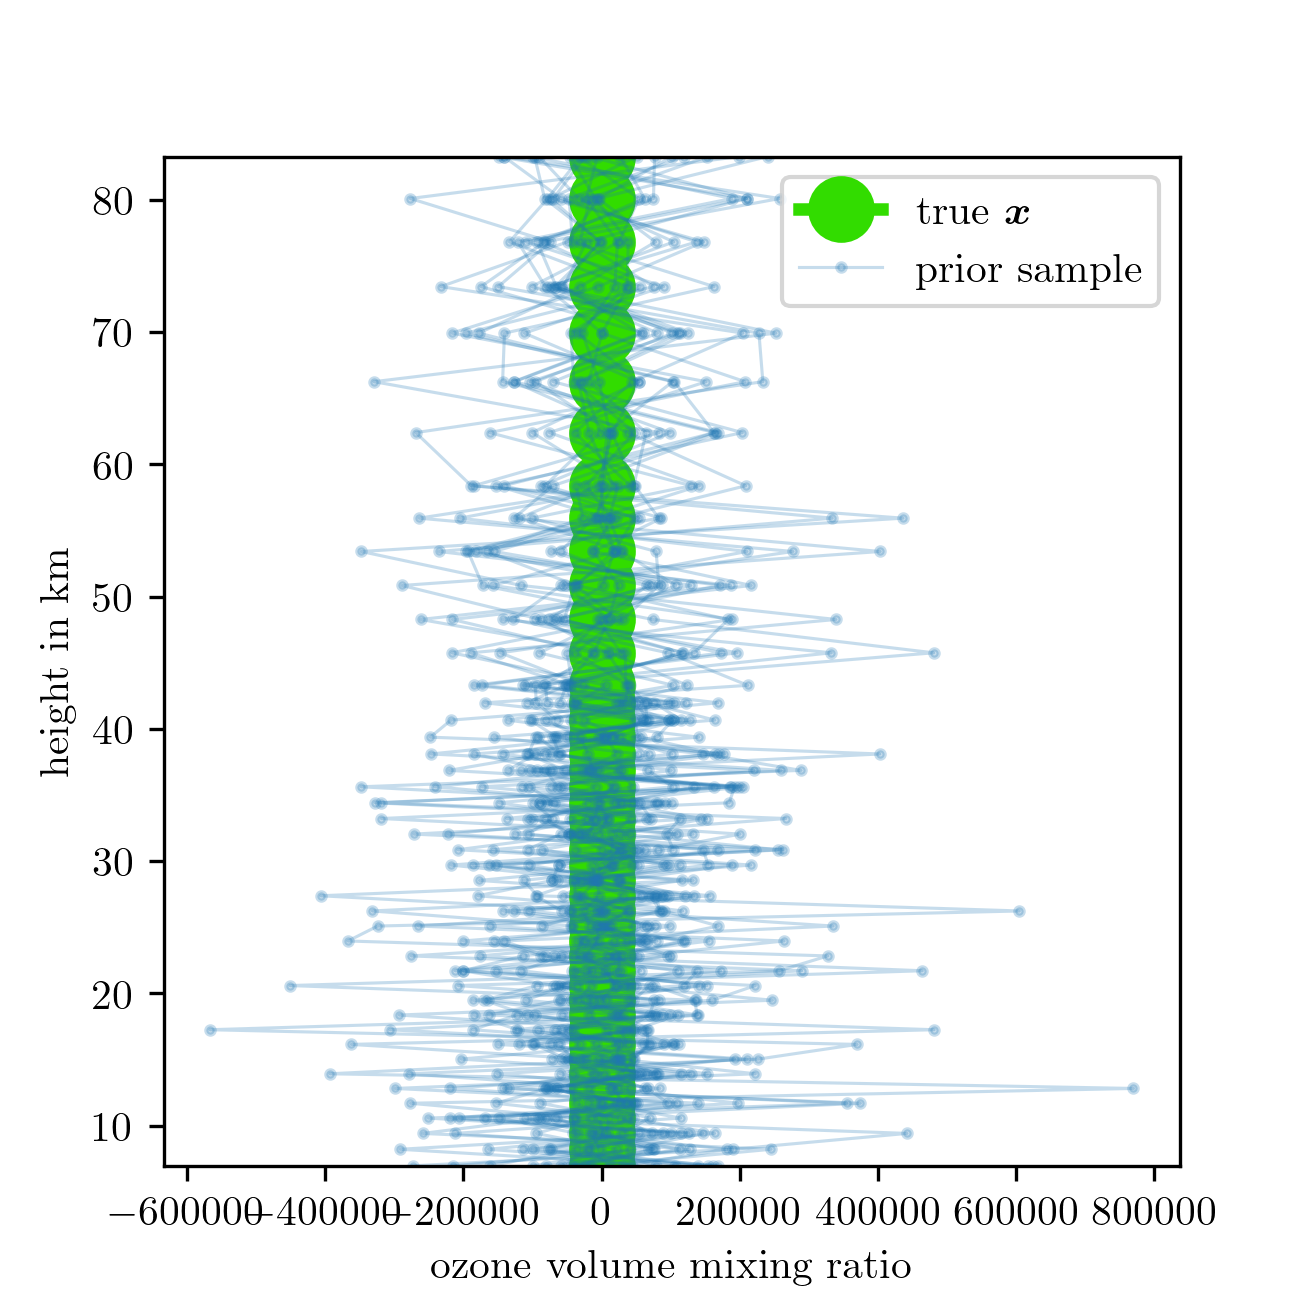
\includegraphics{OzonePrior.png}
	\caption[Samples from ozone prior distribution.]{We draw samples from ozone prior distribution $\bm{x} \sim \mathcal{N}(0,\delta \bm{L})$ after generating a sample from the hyper-prior distribution $\delta \sim \mathcal{T}(1,10^{-10})$. Note that since the spread/variance of prior samples is very large compared to the ozone volume mixing ratios, the ozone profile appears to be constant, which it is not, as seen e.g. in Fig. \ref{fig:O3Samp}.}
	\label{fig:O3Prior}
\end{figure}
\subsubsection{pressure over temperature}
We parametrize the pressure by fitting one exponential to the pressure values $p$ related to the height $h$ by Eq. \ref{}.
We have to be carefull when we choose priors for the tmeprature and pressure

Height priors for temperature don ot overlap also grid for TT is chosen that way

Then pressure prior can not overlap the lowest atmospheric layer as then we would need a second gradient for the exponential

we are also limited by numerical issues of TT
and essentially we can choose uniform priors but then the t-walk would run forever limit parameter space
In case of uniformative data the priors can help us limit the parameter space.

We also show in the appendix that the temperature does not influence the pressure , even though they are correlated
\begin{itemize}
	\item show that pressure is dominant
	\item correlation structure
	\item appendix
\end{itemize}

PriorTempOverPostMeanSigm



\begin{figure}[ht!]
	\centering
	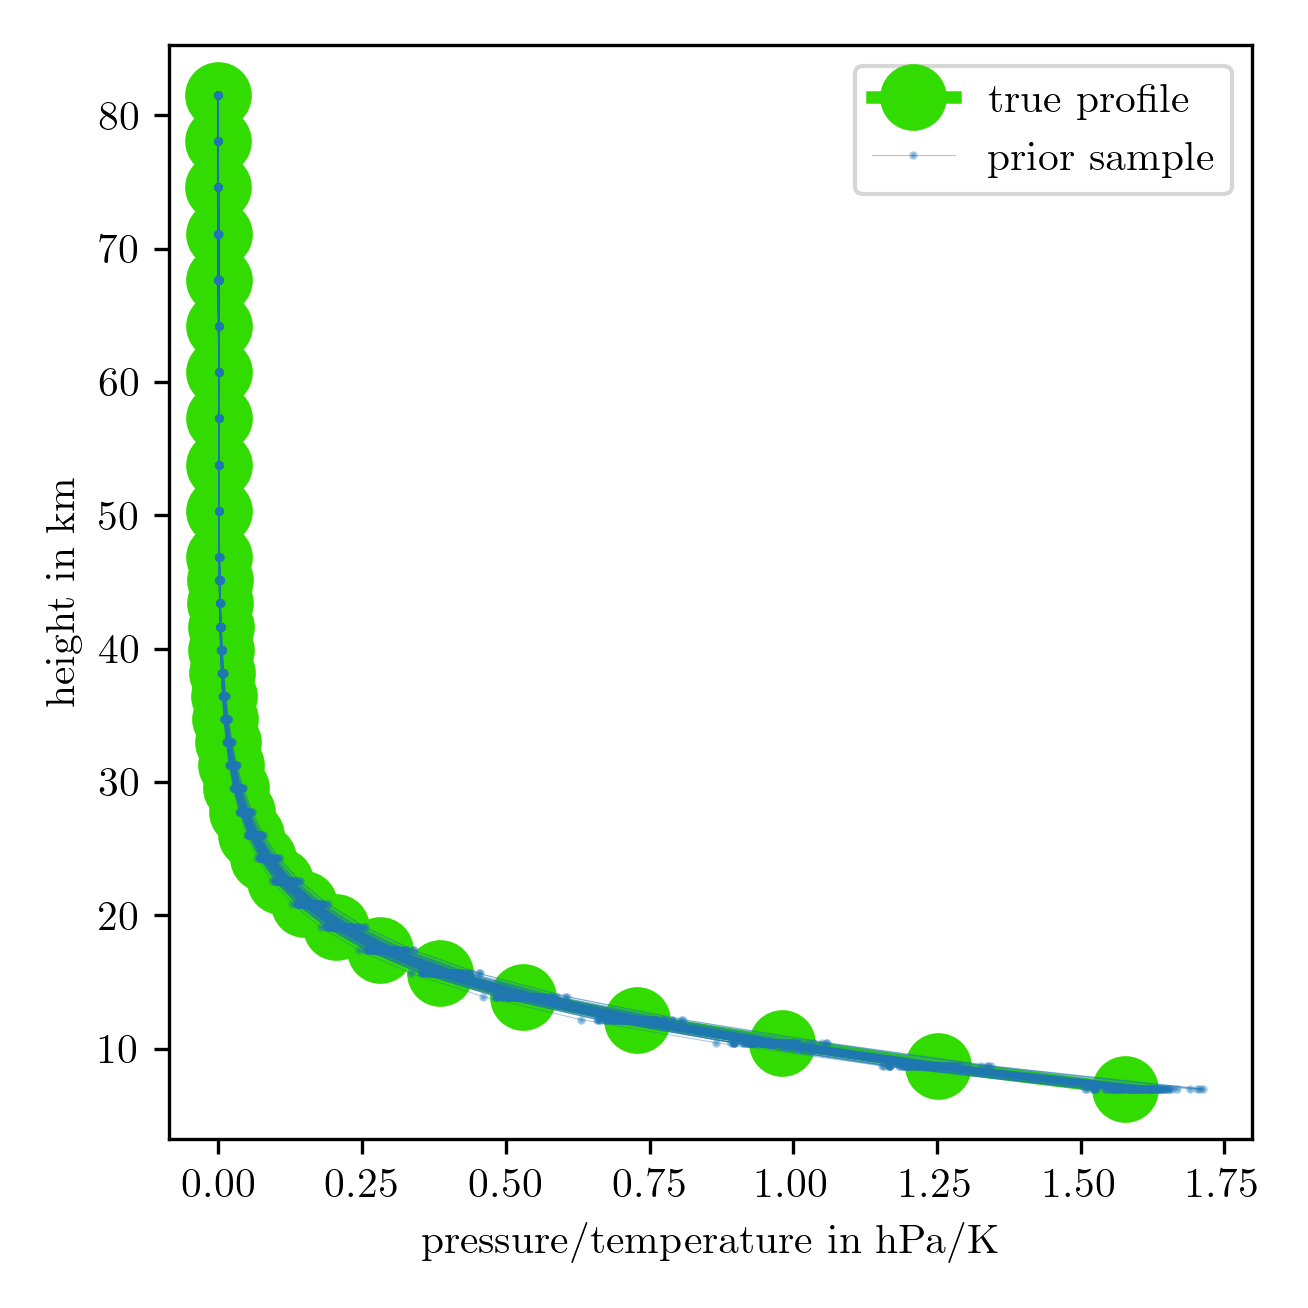
\includegraphics{PriorTempOverPostMeanSigm.png}
	\caption[Prior Samples of $\bm{p}/\bm{T}$ according to the respective hyper-prior distribution.]{We draw samples from the hyper-prior distribution of $h_0, b, p_0, h_1, h_2,h_3,h_4,h_5,h_6, a_0, a_1, a_2,a_3,a_4$ and $T_0$ as defined in table \ref{tab:priors} and then calculate $\bm{p}/\bm{T}$ according to the functions in Eq. \ref{eq:pressFunc} and \ref{eq:tempFunc}.}
	\label{fig:PriorPressOverTemp}
\end{figure}

\begin{figure}[ht!]
	\centering
	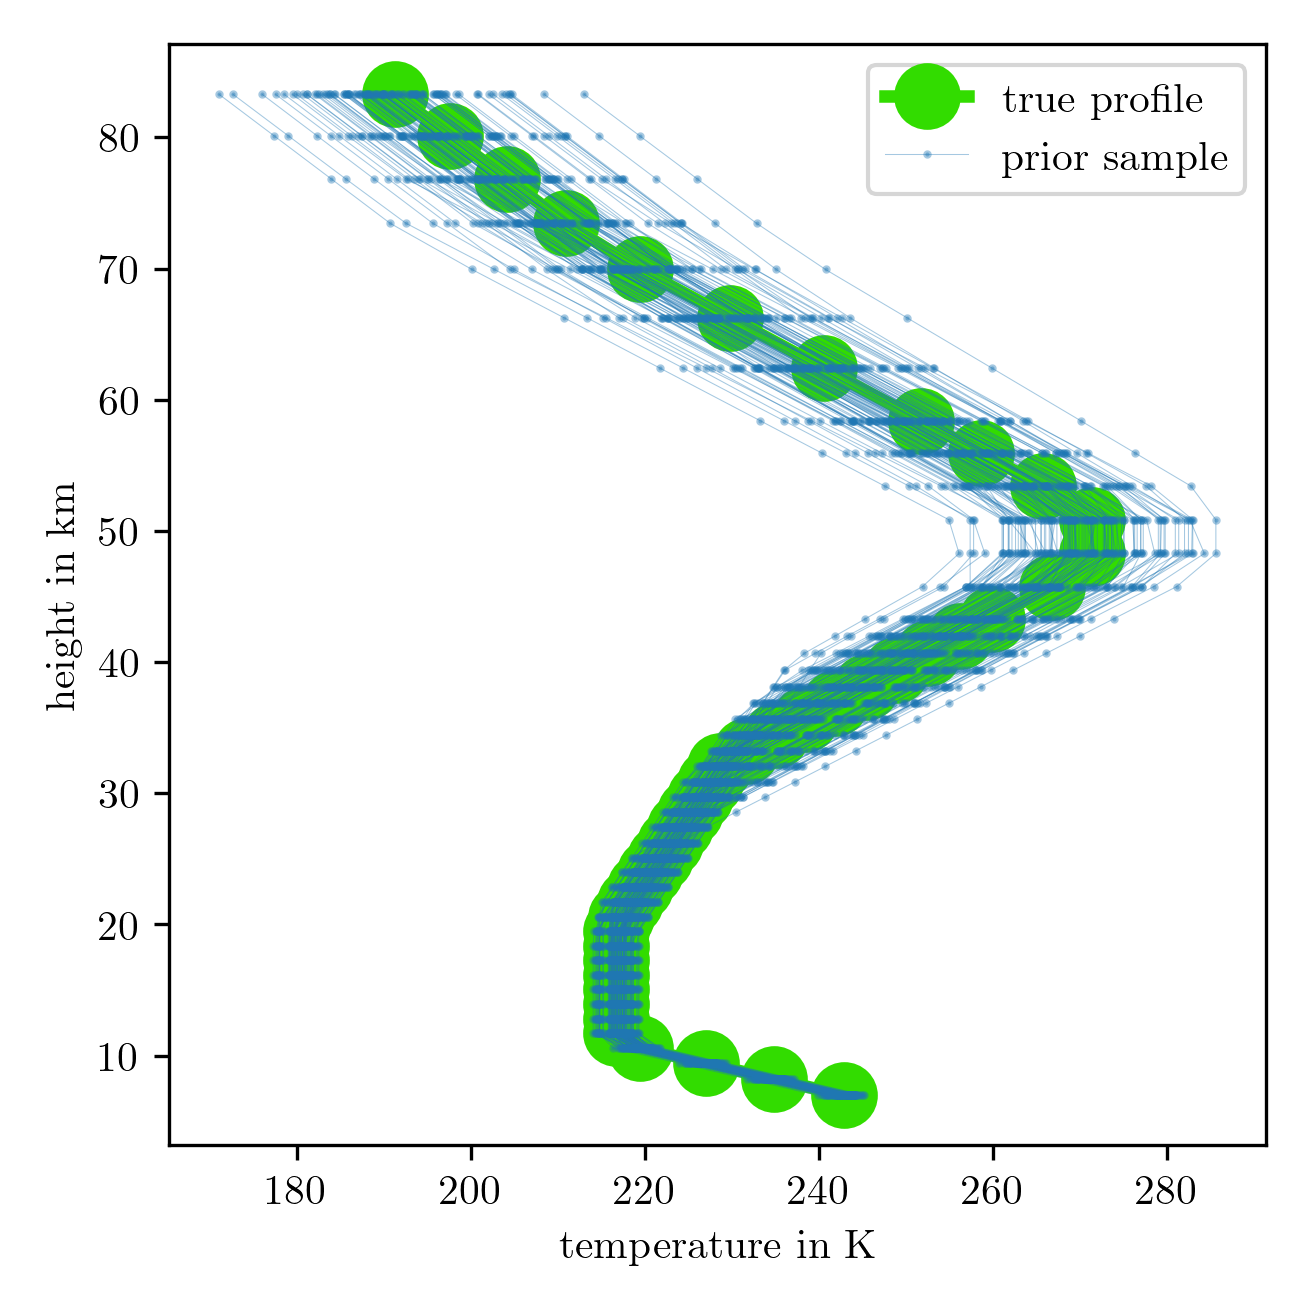
\includegraphics{PriorTempPostMeanSigm.png}
	\caption[Prior Samples of $\bm{T}$ according to the respective hyper-prior distribution.]{We draw samples from the hyper-prior distribution of $h_1, h_2,h_3,h_4,h_5,h_6, a_0, a_1, a_2,a_3,a_4$ and $T_0$ as defined in table \ref{tab:priors} and then calculate $\bm{T}$ according to the function in Eq. \ref{eq:tempFunc}.}
	\label{fig:PriorTemp}
\end{figure}

\begin{figure}[ht!]
	\centering
	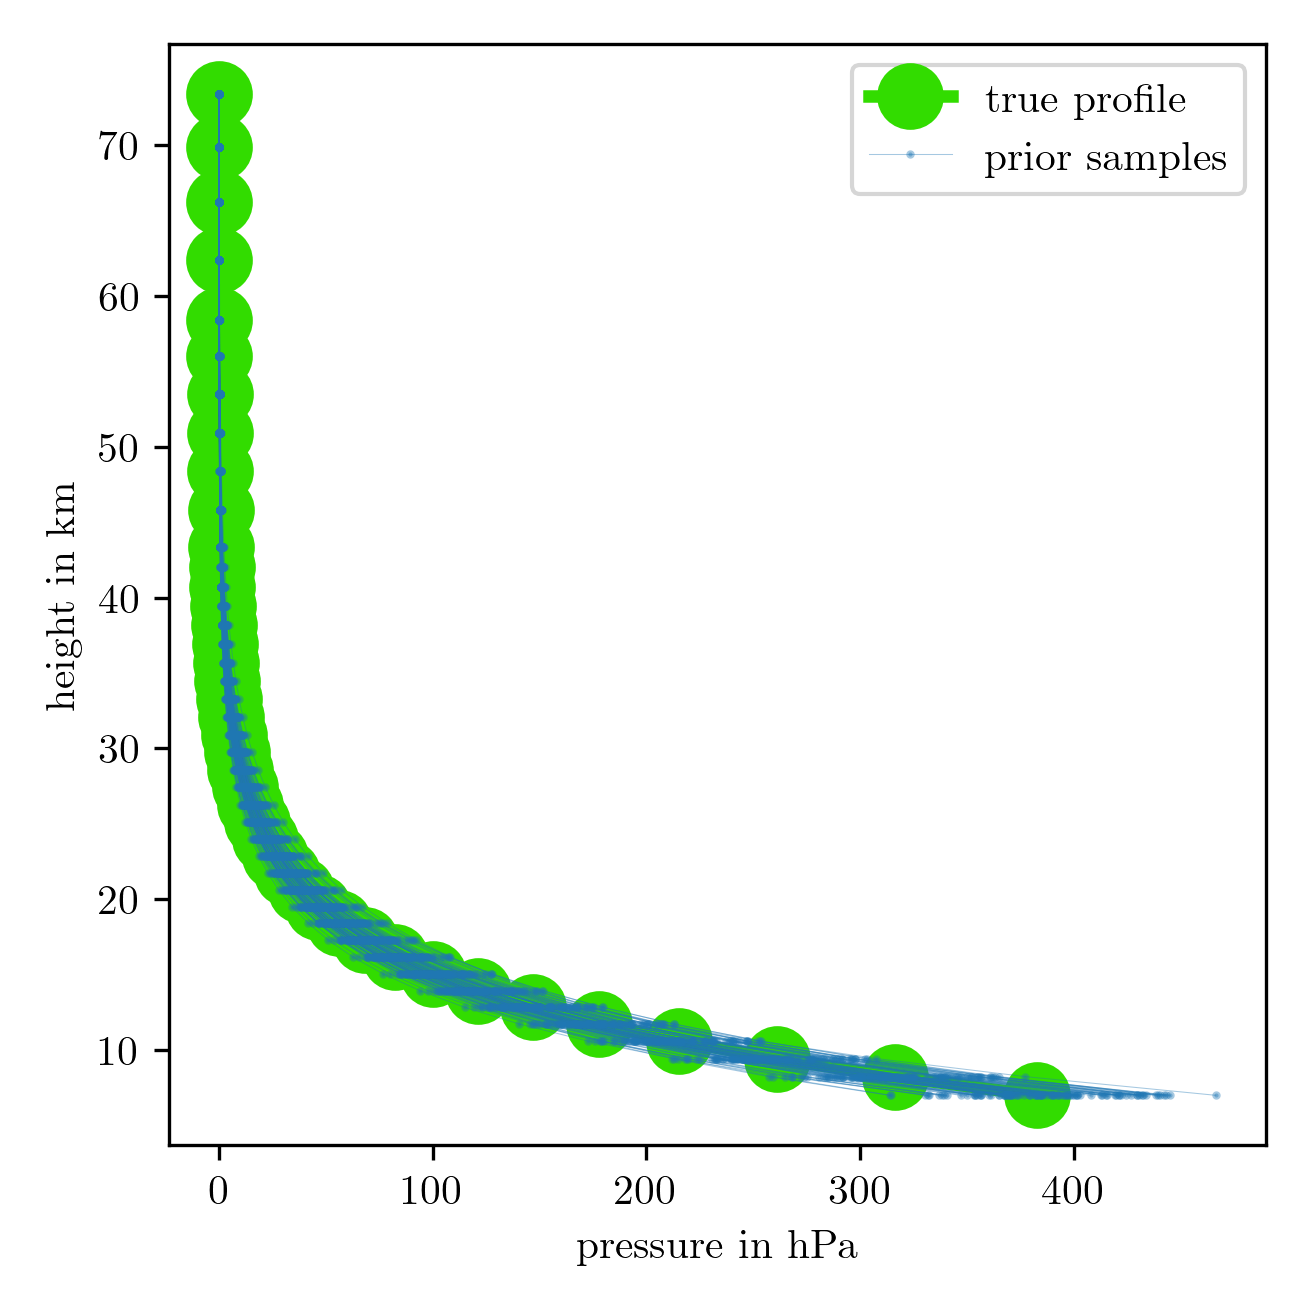
\includegraphics{PriorPressPostMeanSigm.png}
	\caption[Prior Samples of $\bm{p}$ according to the respective hyper-prior distribution.]{We draw samples from the hyper-prior distribution of $h_0, b$ and $p_0$ as defined in table \ref{tab:priors} and then calculate $\bm{p}$ according to the function in Eq. \ref{eq:pressFunc}.}
	\label{fig:PriorPress}
\end{figure}


\section{Posterior distributions with Linear model for Ozone -- MTC}

\begin{itemize}
	\item explain where we use MTC and that T/p is spereate
	\item marginal posterior, noise and covarince and perciosn matrix
	\item picture of f and g
	\item taylor expansion
	\item maybe make  metroplis explixit
\end{itemize}
\begin{figure}[thb!]
	\centering
	\begin{tikzpicture}
		\node[roundnode2] at (-4,6.5) (Q)     {$\bm{Q}$};
		\node[roundnode2] at (-2.5,5) (x)     {$\bm{x}$};
		\node[align=center] at (-1,4) (A)    {$\bm{A}_L$};
		\node[roundnode2] at (-1,2.5) (u)    {$\bm{\Omega}$};
		\node[rectnode] at (-1,1) (y)    {$\bm{y}$};
		\node[roundnode2] at (-2.5,2.5) (e)    {$\bm{\eta}$};
		\node[roundnode2] at (-6.25,6.5) (S)    {$\bm{\Sigma}$};
		\node[roundnode2] at (-7.75,8) (s)    {$\gamma$};
		\node[roundnode2] at (-5.5,8) (d)    {$\delta$};
		
		%Lines
		\draw[->, very thick] (S.south east) -- (e.north west);
		\draw[->, mydotted, very thick] (s.south east) -- (S.north west);
		\draw[->, mydotted, very thick] (e.south east) -- (y.west);
		\draw[->, very thick] (u.south) -- (y.north);
		\draw[->, mydotted, very thick] (A.south) -- (u.north);
		\draw[->, mydotted,  very thick] (x.south east) -- (A.west);
		
		\draw[->, mydotted, very thick] (d.south east) -- (Q.north west); 
		
		\draw[->, very thick] (Q.south east) -- (x.north west); 
		%\node[align=center] at (0,4) (f3) {$= \bm{A}$};
		%\node[align=center] at (0.25,3.95) (f3) {$\approx \bm{M A}_L$};
		\node[align =center] at (-1,7) (T1) {marginal posterior \\ over hyper-parameters \\ $\pi(\gamma, \delta | \bm{y})$};
		\node[align =center] at (0,5) (T1) {conditional posterior \\ $\pi( \bm{x} |\gamma, \delta, \bm{y})$ };
		
		
		\node[fit=(S)(s)(Q)(d),draw,dotted,black, rounded corners] {};
	\end{tikzpicture} 
	\caption[Directed acyclic graph for ozone retrieval and MTC scheme.]{Directed acyclic graph for ozone retrieval and MTC scheme as described in Fig. \ref{fig:DAGComplete}. The hyper-parameters $\delta$ and $\gamma$ determine the noise covariance $\bm{\Sigma}$ for the random noise vector $\bm{\eta} \sim \mathcal{N}(0, \gamma^{-1}\bm{I})$ and the prior precision matrix $\bm{Q} = \delta \bm{L}$ for the distribution over $\bm{x} \sim \mathcal{N}(0, \delta \bm{L})$, where $\bm{L}$ is the graph Laplacian, see Eq. \ref{eq:GLapl}. In the MTC scheme we evaluate the marginal posterior over the hyper-parameters $\pi(\gamma, \delta | \bm{y})$ as in Eq. \ref{eq:} first and then conditional posterior $\pi(\bm{x}|\gamma,\delta,\bm{y})$ as in Eq. \ref{eq:}. The parameter$\bm{x}$ determine the space of all measurable noise free data $\bm{\Omega}$ through the forward model $\bm{A}(\bm{x},\bm{p},\bm{T})$ from which we randomly observe a data set plus some random noise.
		Note that once we found an affine map we update the forward model to $\bm{M}\bm{A}_L$.}
	\label{fig:DAGO3}
\end{figure}

we condition on the pressure and temperature ground truth, ideally we shoul draw a smaple from the posterior distribution 
then we do the MTC scheme whith 

\subsection{Hyper-parameters samples from the marginal posterior distribution}

\begin{figure}[ht!]
	\centering
	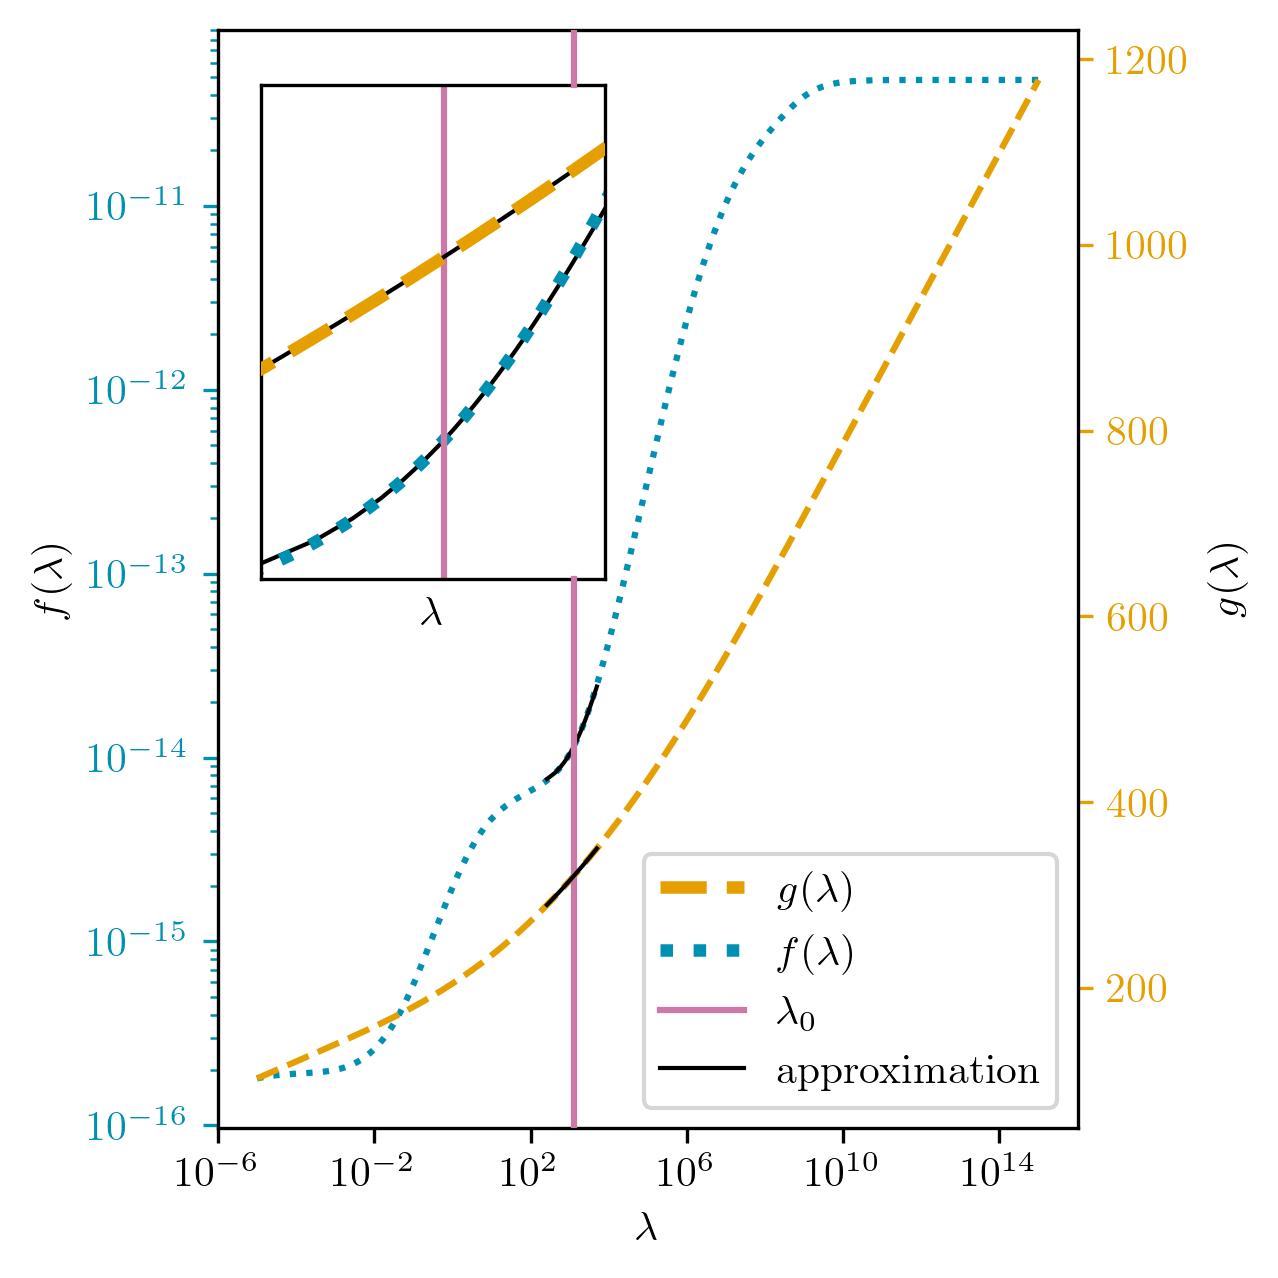
\includegraphics{f_and_g_phd.png}
	\caption[Plot of the functions $f(\lambda)$ and $g(\lambda)$ for marginal posterior.]{Plot of the functions $f(\lambda)$ and $g(\lambda)$ for marginal posterior for a wide range of $\lambda = \delta / \gamma$. We plot the third Taylor series expansion in black around the mode of the marginal posterior (vertical line) for the sampling range of $\lambda$ within the MTC scheme.}
	\label{fig:fandg}
\end{figure}
%In this section we present two algorithm to sample from the marginal posterior distribution.
Now, to sample from the marginal posterior of the hyper-parameters
% and the posterior distribution of the parameters condition on the hyper-parameter $\pi(\bm{x}|\bm{y}, \lambda, \gamma )$, with $\lambda = \delta / \gamma$.
\begin{align}
	\pi(\lambda, \gamma | \bm{y})
	\propto  \lambda^{n/2} \gamma^{m/2}   \exp{ \Bigl\{ - \frac{1}{2} g ( \lambda) - \frac{\gamma}{2} f ( \lambda) \Bigr\} } \pi(\lambda, \gamma),
	\label{eq:MargPostAppl}
\end{align}
with $\lambda = \delta / \gamma$,
\begin{subequations}
	\label{eq:fandg}
	\begin{align}
		&f ( \lambda) = \bm{y}^T \bm{y} - (\bm{A}^T \bm{y})^T (\bm{A}^T  \bm{A} + \lambda \bm{L})^{-1} (\bm{A}^T \bm{y})  \, ,  \\
		&\text{and } g(\lambda) = \log \det (\bm{A}^T  \bm{A} + \lambda \bm{L}) \,.
	\end{align}
\end{subequations}
we employ a so-called MWG (Metropolis within Gibbs) algorithm, summarised in the algorithmic Box $1$.
One may implement a Metropolis random walk on the full conditional
\begin{align}
	\label{eq:lamCondPrior}
	\pi(\lambda | \bm{y}, \gamma) &\propto \lambda^{n/2+\alpha_\delta -1} \exp{\Bigl\{ - \frac{1}{2} g ( \lambda) - \frac{\gamma}{2} f ( \lambda) - \beta_\delta \gamma \lambda \Bigr\}} 
\end{align} 
and do a Gibbs steps on
\begin{align}
	\gamma |  \bm{y}, \lambda &\sim \Gamma \bigg( \frac{m}{2} + \alpha_\delta + \alpha_\gamma, \frac{1}{2} f (\lambda ) + \beta_\gamma + \beta_\delta \lambda \bigg)\label{eq:gamCondPrior}
\end{align} 
to generate marginal posterior samples $(\lambda, \gamma)^{(1)}, \dots, (\lambda, \gamma)^{(N)} \sim  \pi(\lambda, \gamma| \bm{y})$.
Note that, when changing variables from $\delta = \lambda \gamma$ to $\lambda$ the hyper-prior distribution changes to $\pi(\lambda) \propto \lambda^{\alpha_\delta-1} \gamma^{\alpha_\delta} \exp{(- \beta_\delta \lambda  \gamma)} $, due to $\text{d}\delta / \text{d} \lambda = \gamma$.
We find the full conditionals by factorisation.



\begin{align} 
	\log \left\{ \frac{\pi(\lambda | \gamma^{(t-1)}, \bm{y})  }{\pi(\lambda^{(t-1)}| \gamma^{(t-1)}, \bm{y})}  \right\} 
	= \log  \{\pi(\lambda | \gamma^{(t-1)}, \bm{y} ) \}  -\log  \{ \pi(\lambda^{(t-1)}| \gamma^{(t-1)}, \bm{y}) \} \\
	= \frac{n}{2} (\log\{\lambda\} - \log\{\lambda^{(t-1)}\} ) + \frac{1}{2} \Delta g + \frac{\gamma^{(t-1)}}{2} \Delta f  + \beta_\delta \gamma^{(t-1)} \Delta \lambda  
\end{align}
As part of the Metropolis random walk, a new $\lambda^\prime$ given the previous $\lambda^{(k)}$, with $k = 1 , \dots, N$, is proposed according to the distribution $q(\lambda^\prime|\lambda^{(k)}) \sim \mathcal{N}(\lambda^{(k)}, w_\lambda)$.
The proposed sample is rejected or accepted with the acceptance probability $\alpha(\lambda^\prime |\lambda^{(k)})$, see Equation \eqref{eq:alpha}.
Here, calculating the difference $\Delta f = f(\lambda^\prime) - f(\lambda^{(k)})$ and $\Delta g = g(\lambda^\prime) - g(\lambda^{(k)})$ is crucial.
Since the functions $f(\lambda)$ and $g(\lambda)$ are well-behaved over a large range of $\lambda$ and almost linear around the mode of the marginal posterior $\lambda_0$, a Taylor expansion around the mode is sufficient, see Figure \ref{fig:f_and_g}.
Then, computing the acceptance ratio does not involve evaluating $f(\lambda)$ and $g(\lambda)$, but the difference $\Delta f = \sum f^{(r)}(\lambda_0) (\Delta \lambda^\prime - \Delta \lambda^{(k)})^r$ and $\Delta g = \sum g^{(r)}(\lambda_0) (\Delta \lambda^\prime - \Delta \lambda^{(k)})^{r}$, where $\Delta \lambda^\prime = \lambda^\prime - \lambda_0 $ and $\Delta \lambda^{(k)} =  \lambda^{(k)} - \lambda_0$
The derivatives are
\begin{align}
	f^{(r)}& (\lambda_0)= (-1)^{r+1} r! (\bm{A}^T \bm{y})^T (\bm{B}_0^{-1} \bm{L})^r \bm{B}_0^{-1} \bm{A}^T \bm{y} \label{eq:ftay}  \\
	\text{and } &g^{(r)} ( \lambda_0) = (-1)^{r+1} \, \text{tr} \big( (\bm{B}_0^{-1}\bm{ L })^r \big)
	\label{eq:gtay}
\end{align} 
with $\bm{B}_0 = \bm{A}^T  \bm{A} + \lambda_0 \bm{L}$.

Finally, a Gibbs step provides a new $\gamma^{(k+1)} \sim \gamma | \bm{y}, \lambda^{(k+1)}$, see Equation \eqref{eq:GibbsStep}.
\begin{figure}[ht!]
	\centering
	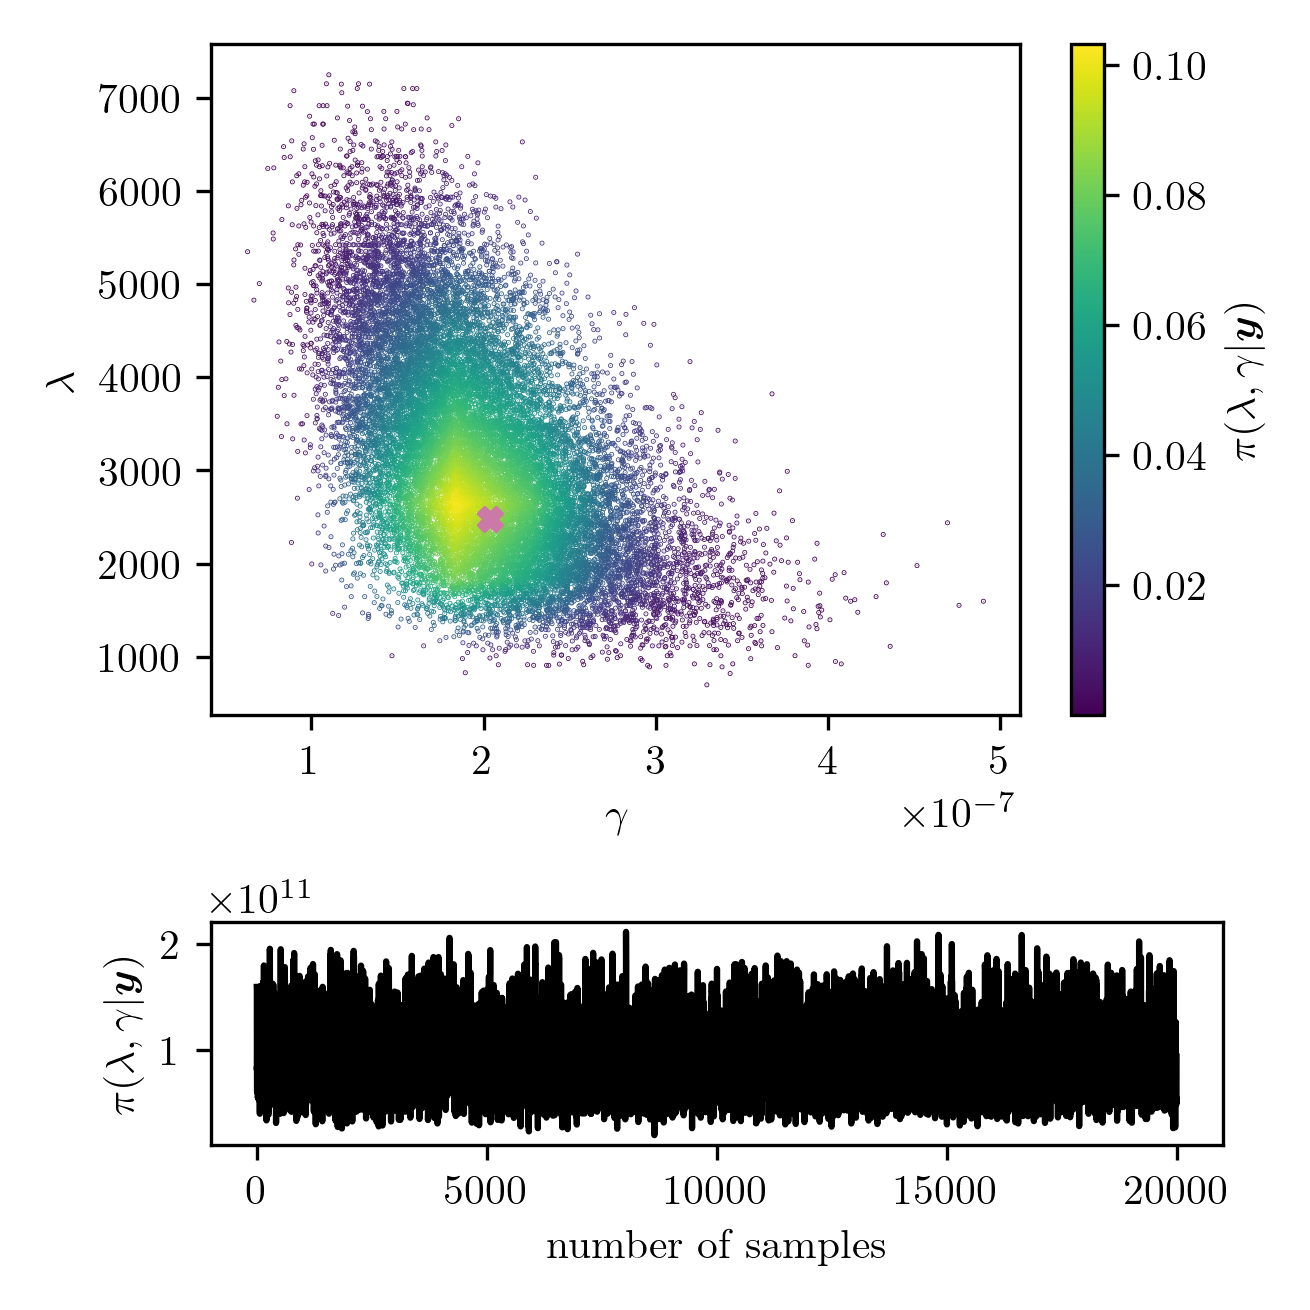
\includegraphics{ScatterplusHistoPlusTT.png}
	\caption[Scatter plot of samples from marginal posterior, including weighting from TT approximation; additional trace plot of the marginal posterior samples.]{We scatter plot the samples of $\lambda = \delta / \gamma $ and $\gamma$ from the marginal posterior $\pi(\lambda , \gamma  | \bm{y})$ and colour code the samples using the TT approximation of $\pi(\lambda , \gamma  | \bm{y})$. To show ergodicity we plot the trace of the samples of the Metropolis-within-Gibbs sampler below.}
	\label{fig:ScatterPlotTT}
\end{figure}

\begin{algorithm}[!ht]
	\caption{Metropolis within Gibbs for $\pi(\lambda, \gamma | \bm{y})$}
	\begin{algorithmic}[1]
		\STATE Initialise  \( \bm{\theta}^{(0)}  =( \lambda^{(0)} , \gamma^{(0)}  ) \) and set burn-in $N_{\text{burn-in}}$
		\FOR{ \( k = 1, \dots, N^{\prime} \)}
		\STATE Propose \( \lambda \sim \mathcal{N}(\lambda^{(t-1)}, 0.8 \lambda_0)  \)
		\STATE Compute
		\[ \alpha( \lambda  | \lambda^{(t-1)}) = \min \left\{ 1, \frac{\pi(\lambda | \gamma^{(t-1)}, \bm{y})  }{\pi(\lambda^{(t-1)}| \gamma^{(t-1)}, \bm{y})}  \right\} \]
		\STATE Draw $u \sim \mathcal{U}(0,1)$
		\IF{$\alpha \geq u$ }
		\STATE Accept and set \( \lambda^{(t)} = \lambda \)
		\ELSE  
		\STATE Reject and keep \(\lambda^{(t)} = \lambda^{(t-1)} \)
		\ENDIF
		\STATE Draw $\gamma^{(t)} | \lambda^{(t)} ,\bm{y} \sim \text{Gamma} \big( 0.5  \, m + 2, 0.5 \, f(\lambda^{(t)}) + 10^{-10}(1 + \lambda^{(t)}) \big) $
		\ENDFOR
		%\STATE Output: $ \bm{\theta}^{(N_{\text{burn-in}})}, \dots,  \bm{\theta}^{(k)} , \dots,   \bm{\theta}^{(N)} \sim \pi(\bm{\theta}| \bm{y}) $
		\STATE Output: $ (\lambda, \gamma)^{(N_{\text{burn-in}})}, \dots,  (\lambda, \gamma)^{(k)} , \dots,   (\lambda, \gamma)^{(N)} \sim \pi(\lambda, \gamma| \bm{y}) $
	\end{algorithmic}
\end{algorithm}

\subsection{Ozone samples from the conditional posterior}
Two ways
treat is as truncated multivariate normal distribution
\subsubsection{RTO}
Conditioned on the hyper-parameters $\bm{\theta} = ( \delta, \gamma)$ we utilise the so-called RTO (randomize then optimize) method \cite{bardsley2012mcmc,bardsley2015randomize, fox2016fast} to draw an independent sample of the conditional posterior distribution.
By perturbation of the exponent of
\begin{align}
	\bm{x}| \bm{y} ,\delta, \gamma \sim \mathcal{N}\big( \underbrace{ (\bm{A}^T \bm{A} + \delta / \gamma \bm{L} )^{-1} \bm{A}^T \bm{y}}_{\bm{x}_{\lambda}}, (\gamma \bm{A}^T \bm{A} + \delta \bm{L} )^{-1} \big) \, \label{eq:CondPost},
\end{align}
we obtain one independent sample $\bm{x} \sim \pi(\bm{x}|\bm{y}, \bm{\theta})$ for each solve of Equation \eqref{eq:RTO}, see algorithmic Box $2$.


We use the same discretization of the atmosphere as given by the ozone profile taken from \cite{MLSdata} \url{https://disc.gsfc.nasa.gov/datasets/ML2O3_005/summary?keywords=mls%20o3}.
We use ozone values between a height of $10$km up to $38$km, which results in $n=37$ layers.
We set the number of measurements to $m= 105 $.
(I can't think of any good reason why I chose that, it is a good number not too big not too small and gives consistent results for various datasets)\\

When finding the mode we use the scipy.optimize.fmin function and limit the number of function evaluations to 25.
We use Cholesky factorisation to evaluate $g(\lambda)$ and $f(\lambda)$ and to construct the coefficients of the Taylor series, where we have to calculate  $\bm{B}^{-1} \bm{L} $ and  $\bm{B}^{-1}  \bm{A}^T \bm{y}$ once at $\lambda_0$.\\

\subsubsection{Weighted Mean}
We bin the samples into a normalised histogram and use the height of the bars as quadrature weights $\pi(\lambda_i| \bm{y})$, where the quadrature point $\lambda_i$ denotes the centre of each bin.
To calculate the conditional posterior mean we use approximate quadrature
\begin{align}
	\mu_{\bm{x}|\bm{y}} = \int \bm{x}_{\lambda} \pi(\lambda| \bm{y}) \text{d}\lambda \approx \sum \bm{x}_{\lambda_i} \pi(\lambda_i| \bm{y}) \, ,
\end{align}
with $\sum \pi(\lambda_i| \bm{y}) = 1$, so that the integral can be interpreted as the weighted average.
See Sec. 2.1
\cite{Dick_Kuo_Sloan_2013} \url{https://www.cambridge.org/core/journals/acta-numerica/article/highdimensional-integration-the-quasimonte-carlo-way/03F126DDF465F915B22D5D709CD28946}.\\

We bin the samples into $3$ bins and stop increasing the number of bins by one if the relative error between the previous and the current conditional posterior mean is less than $0.1\%$.
This gives a total number of $3+4+5 = 12$ solves for $x_{\lambda}$.
In addition, we calculate the covariance matrix $(\gamma \bm{B}_{\lambda})^{-1} $, where we use Cholesky factorisation to invert $\bm{B}$, solving the integral
\begin{align}
	\Sigma_{\bm{x}|\bm{y}} = \int \gamma^{-1}  \pi(\gamma | \bm{y} ) \, \text{d} \gamma \, \int  \bm{B}_{\lambda}^{-1} \, \pi(\lambda | \bm{y} )  \, \text{d} \lambda  \approx \sum {\gamma_i}^{-1}\pi(\gamma_i| \bm{y}) \sum \bm{B}_{\lambda_i}^{-1}\pi(\lambda_i| \bm{y})\, .
\end{align}\\

It takes us less than 0.1s to draw 10000 samples from the marginal posterior and to calculate the conditional posterior mean or to solve for 200 different $x_{\lambda}$ and to find the regularised solution at the point of maximum curvature using the kneedle algorithm.\\

\begin{figure}[ht!]
	\centering
	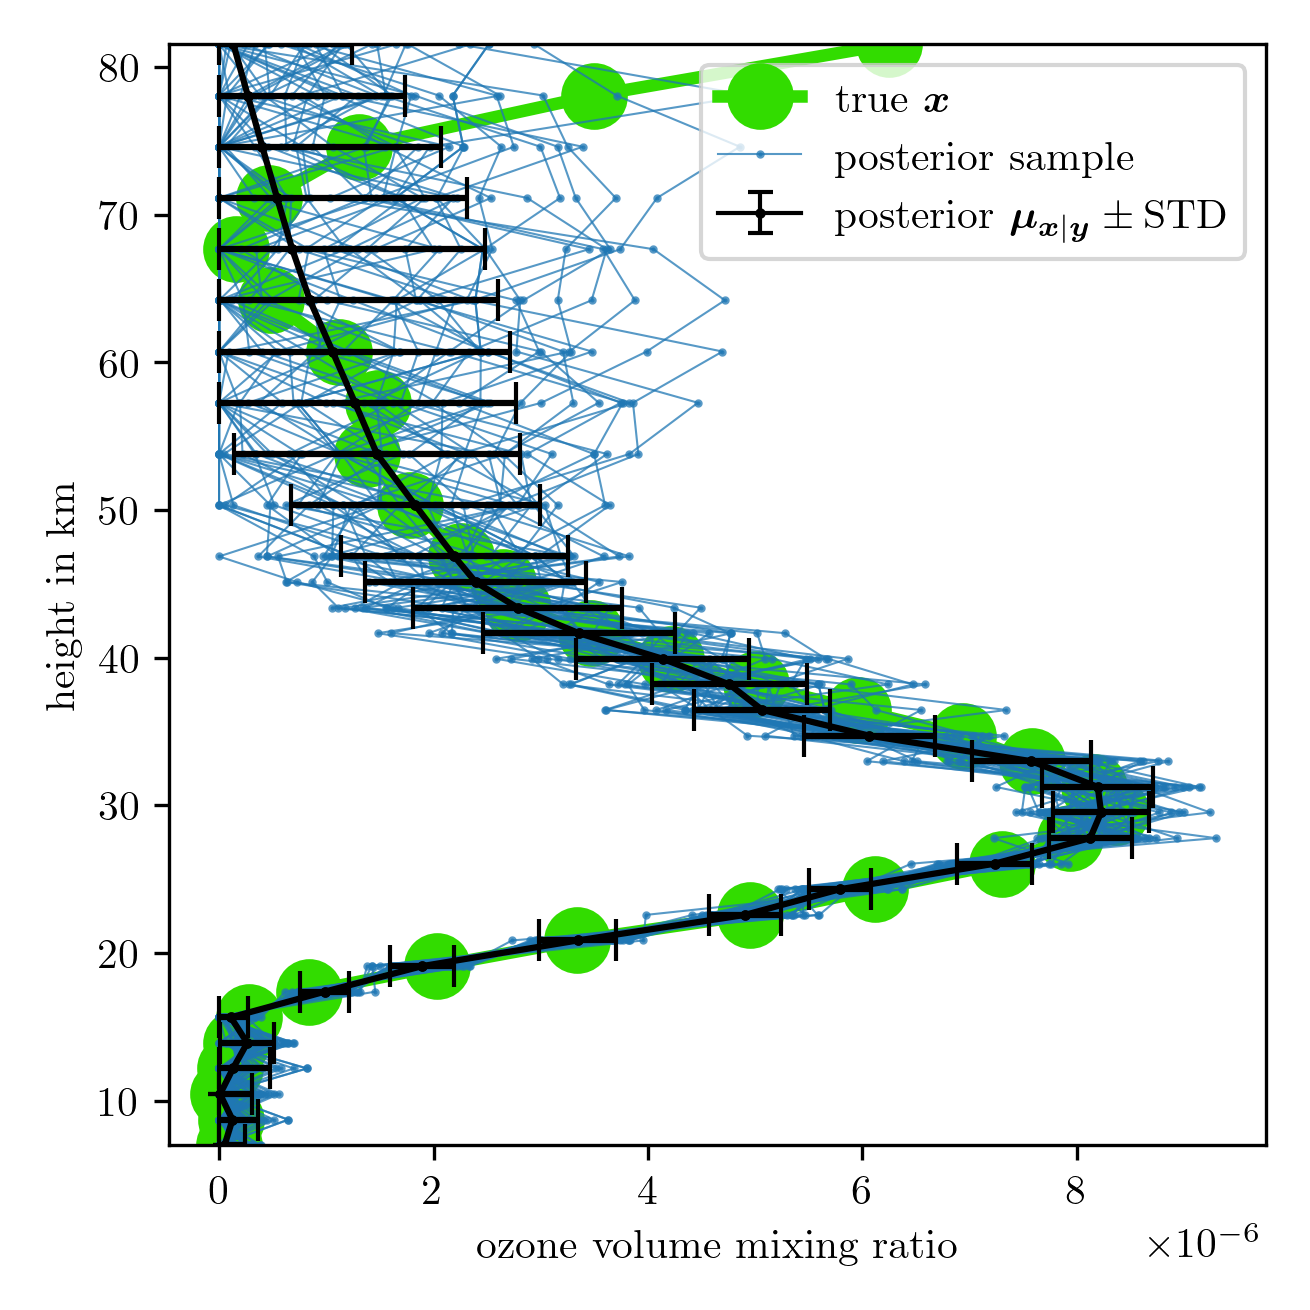
\includegraphics{FirstTestRes.png}
	\caption[Ozone samples of the conditional posterior.]{We draw samples from the conditional posterior distribution  $\pi(\bm{x}|\lambda,\gamma , \bm{y})$ after characterising the marginal posterior $\pi(\lambda,\gamma | \bm{y})$ through sampling or TT approximation using the linear forward map $\bm{A}_L$. We will use those samples to find the affine map $\bm{M}$, see section \ref{sec:affineMap}}
	\label{fig:O3Samp}
\end{figure}

\section{Approximate non-linear forward model with affine Map} 
\label{sec:affineMap}
\begin{itemize}
	\item introduce affine sapce and how we get affine map, to motivate samples from posterir space
	\item explicit, why we need ozone profiles, because it is faster and temperature and pressure are more well defined within the atmosphere
	\item generate affine space every samples is a feasable sample
	\item generate data without noise to find affine map
\end{itemize}

\begin{figure}[thb!]
	\centering
	\begin{tikzpicture}
		\node[rectnode] at (0,0) (Oy)    {$\bm{y}$};
		\node[roundnode2] at (0,-2) (x)     {$\bm{x}$};
		\node[rectnode] at (-1.5,-4) (NLy)    {$\bm{A}_{NL}\bm{x}$};
		\node[rectnode] at (1.5,-4) (y)    {$\bm{A}_L\bm{x}$};
		\draw[->, very thick] (Oy.south) -- (x.north); 
		\draw[->, very thick] (x.south west) -- (NLy.north); 
		\draw[->, very thick] (x.south east) -- (y.north); 
		\draw[->, very thick] (NLy.east) -- (y.west); 
		\node[align=center] at (1,0) (l1) {Data};
		\node[align=center] at (2,-2) (f2) {Ozone Profiles};
		
		\node[align=center] at (-4,-4) (f3) {non-linear forward model};
		\node[align=center] at (4,-4) (f4) {linear forward model};
		\node[align=center] at (0,-5) (f5) {$\bm{A}_{NL} \approx \bm{M A}_L= \bm{A}$ };
		
		\node[align=center] at (0,-4) (f5) {affine Map \\ $\bm{M}$};
		
	\end{tikzpicture}
\end{figure}


We do MTC with linear forward map no updadeted
In this specific case we find the affine map
\begin{align}
	\bm{M} = \begin{bmatrix}
		\text{---} & \bm{M}_0 &   \text{---}  \\
		&  \vdots  & \\
		\text{---}& \bm{M}_j &  \text{---} \\
		&  \vdots  & \\
		\text{---} & \bm{M}_m &   \text{---}
	\end{bmatrix} \, \in \mathbb{R}^{m \times m} ,
\end{align}
with rows $\bm{M}_j$ using a linear solver for
\begin{align}
	W \bm{M}_j^\top \, = V_{j} \, .
\end{align}
Here $V_j$ denotes the $j$th row of  
\begin{align}
	V = \begin{bmatrix}
		\vert&   &  \vert & & \vert \\
		\bm{A}_{NL} (\bm{x}^{(1)} ) &  \cdots& \bm{A}_{NL} (\bm{x}^{(j)} )&  \cdots & \bm{A}_{NL} (\bm{x}^{(m)})  \\
		\vert&   &  \vert & & \vert 
	\end{bmatrix}
\end{align}
and
\begin{align}
	W = \begin{bmatrix}
		\vert&   &  \vert & & \vert \\
		\bm{A}_{L} \bm{x}^{(1)} &  \cdots& \bm{A}_{L} \bm{x}^{(j)} &  \cdots & \bm{A}_{L} \bm{x}^{(m)} \\
		\vert&   &  \vert & & \vert 
	\end{bmatrix}
\end{align}
is a $\mathbb{R}^{m \times m} $ matrix as well as $\bm{A}_{NL}$.
Then the non-linear forward model can be approximated so that
\begin{align}
	\bm{A}_{NL}(\bm{x}) \approx \bm{M A}_L \bm{x}\, .
\end{align}

\begin{figure}[ht!]
	\centering
	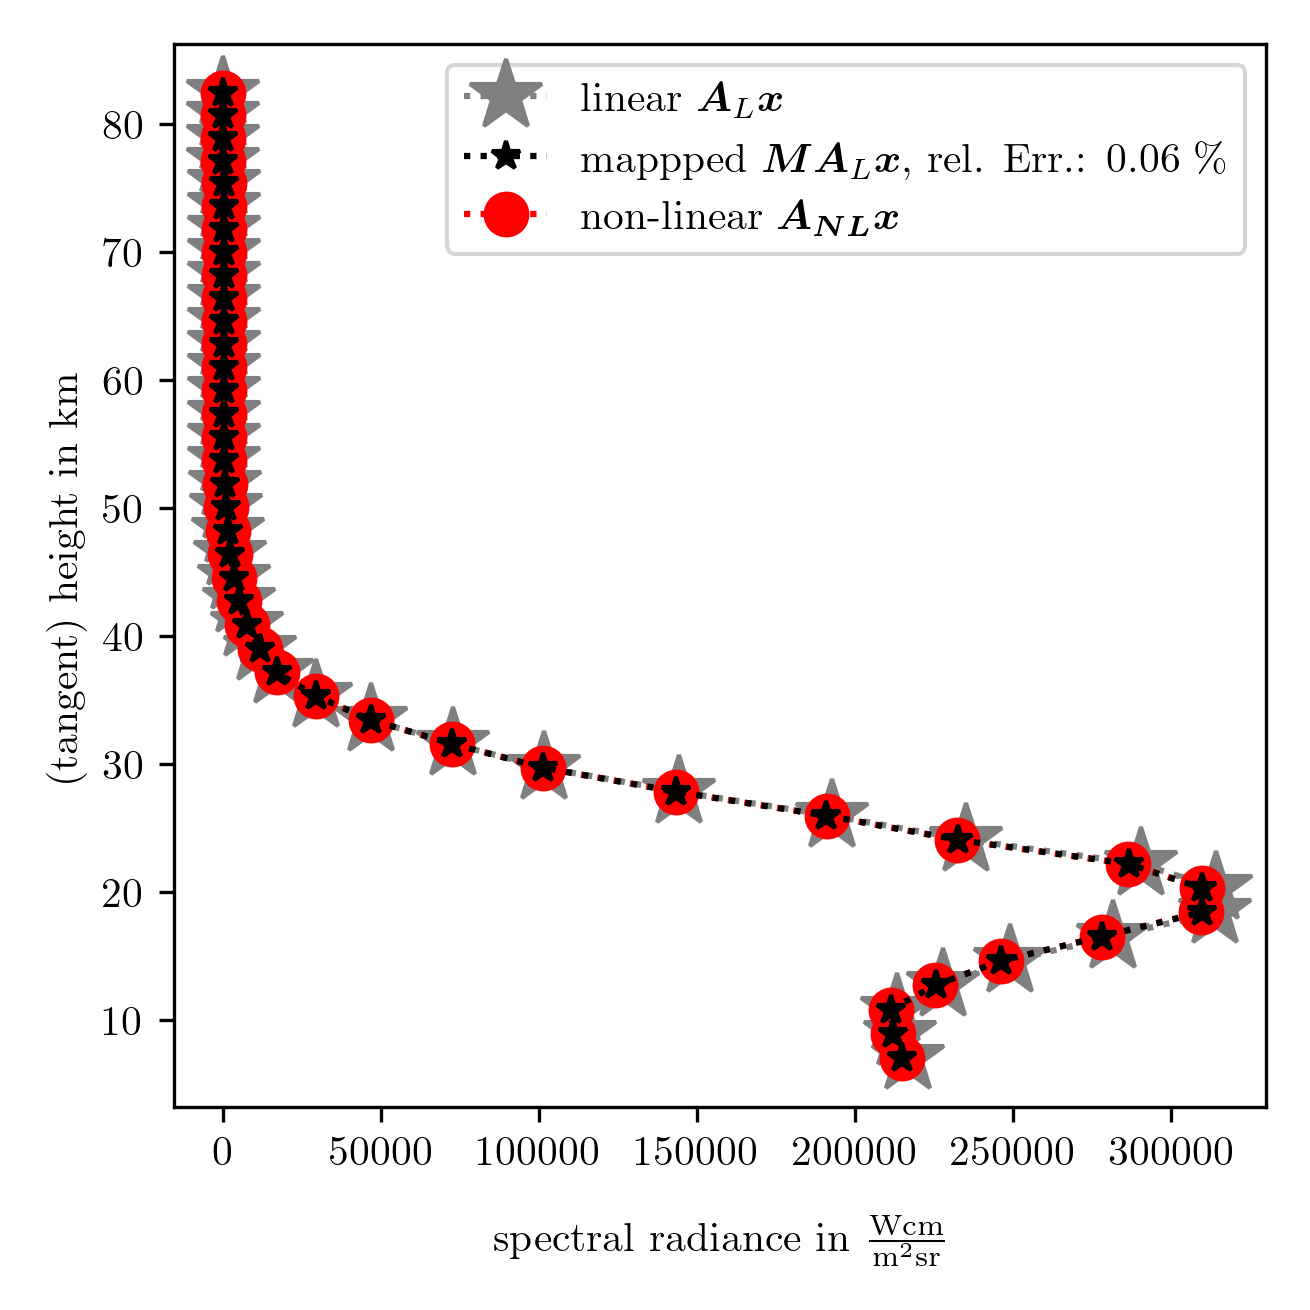
\includegraphics{SampMapAssesment.png}
	\caption[Assessment of affine map.]{We asses how good we can map the linear forward model onto the non-linear forward model using the previous calculated affine map. The gray stars represent noise free linear data, where as the red circles present noise free non-linear data. Then we map the linear noise free data onto the non-linear noise free data and give the relative error in between the mapped noise free data and the non-linear data. the  needs M}
	\label{fig:MapAsses}
\end{figure}


\begin{itemize}
	\item updated forward map
	\item do mtc again but this time with weighted integration and then condition on pressure and temperature, samples
	\item for sake of completeness regularised solution and say disadvantage, maybe include in table
\end{itemize}

\section{Posterior distributions with approximated non-linear model for Ozone -- MTC}
\subsection{Hyper-parameters samples from the marginal posterior distribution}
\begin{figure}[ht!]
	\centering
	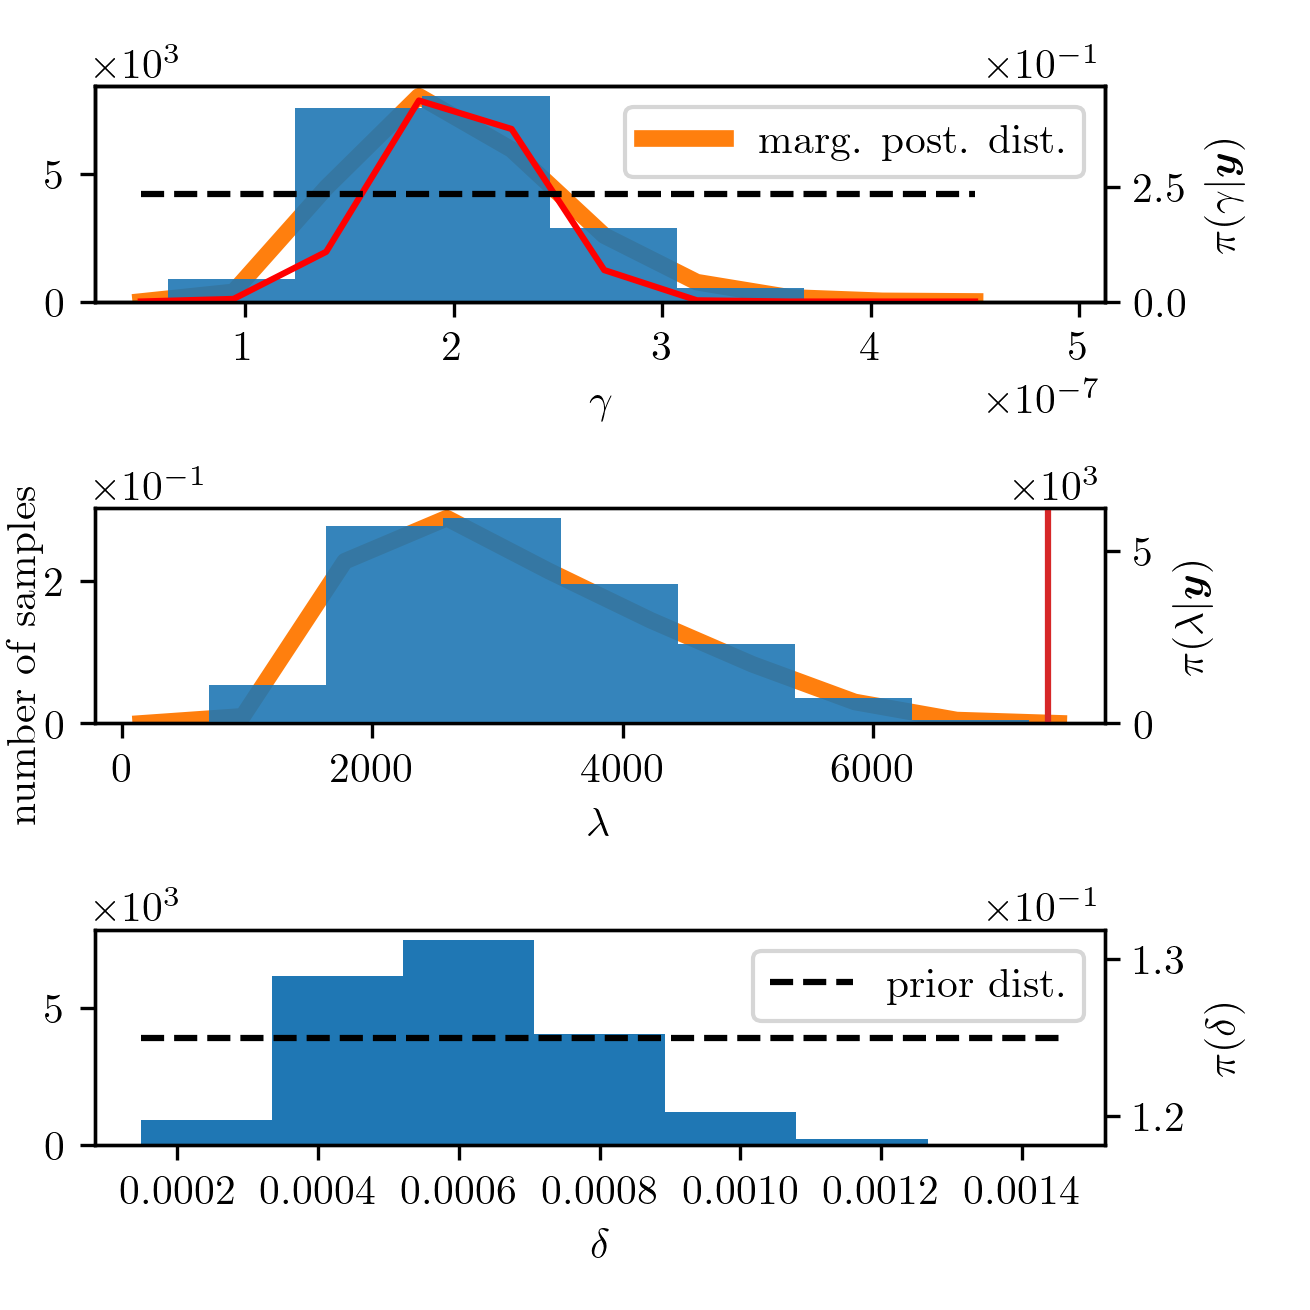
\includegraphics{secSIRTMargMargO3Res.png}
	\caption[Marginal posterior histograms and TT approximation as well as hyper-prior distribution.]{We plot the TT approximation of marginal posterior in orange and the samples as a histogram as well as the prior distribution with a dotted line. Note that we sample $\lambda$ and $\gamma$ using the Metropolis-within-Gibbs sampler and can calculate $\delta$ for every sample of the marginal posterior, we can not do this for the TT approximation. The regularised parameter corresponding to the regularised solution is marked thought the red vertical line at $\lambda_{\text{reg}} =$.}
	\label{fig:MargPostHistTT}
\end{figure}

\begin{itemize}
	\item make table with set up for TT and sampling , number of samples
	\item normalize in evrey step
	\item we use RTO to generate samples
\end{itemize}



\begin{itemize}
	\item samples vs calc values
	\item taylor expansion
\end{itemize}





\subsection{Ozone samples from the conditional posterior and regularised solution}
\begin{itemize}
	\item draw samples using RTO no need to calc variance yet, when variance is hard to calculate, we use Cholesky defactorization (maybe put in appendix)
	\item or calc mean and variance using see other section
\end{itemize}



\subsection{Regularized Solution}
\begin{itemize}
	\item similar to MTC model
	\item picture of L-Curve and samples 
	\item include in reg paraemter in histograms
\end{itemize}

\section{Solution by regularization} \label{sec:reg}
The Tikhonov regularized solution is defined as~\cite{hansen2010discrete} 
\begin{align}
	\bm{x}_{\lambda} =\underset{ \bm{x}}{\arg \min}\,  \lVert \bm{A}\bm{x} - \bm{y} \rVert_2^2 + \lambda \bm{x}^T \bm{L} \bm{x} \, ,
	\label{eq:XLam}
\end{align}
which is equivalent to minimizing the term $T(\bm{x})$ in Equation~\eqref{eq:posterior} with $\lambda = \delta / \gamma$. This maximizes the full conditional distribution for $\bm{x}$, so is not, as often erroneously stated, the maximum a posteriori (MAP) estimate. The regularized solution is typically calculated by solving the normal equations 
%Differentiation and zero setting lead to the regularised ozone profile
\begin{align}
	\bm{x}_{\lambda} = (\bm{A}^T\bm{A} + \lambda \bm{L} )^{-1} \bm{A}^T \bm{y} \label{eq:xLam} \, 
\end{align}
with a separate procedure used to determine the regularizing parameter $\lambda$; in Section~\ref{sec:reg} we demonstrate the L-curve method~\cite{hansen1993use}.
% Here $\bm{x}_\lambda$ maximizes the function $- \ln \pi (\bm{x} | \bm{y}) $ and is also known as the maximum a posterior (\textbf{MAP}) estimator of the non-hierarchical Bayesian model.
% In literature one often refers to the Tikhonov regularization \cite{tikhonov1963regularization}.
\subsection{Regularization}
\label{sec:reg}
According to \cite{hansen1993use}, the regularized solution corresponds to the corner on the L-curve, the point of maximum curvature.
As done in \cite{hansen1993use}, we compute $\bm{x}_\lambda$, see Equation \eqref{eq:xLam}, for 200 different $\lambda$ values and plot the solution semi norm $\sqrt{\bm{x}_\lambda^T\mathbf{L} \bm{x}_\lambda}$ against the data misfit norm $\lVert \bm{A}\bm{x}_\lambda - \bm{x} \rVert$, see Figure \ref{fig:RegCurv}.
We find the point of maximum curvature with the kneedle algorithm~\cite{satopaa2011kneedle} using the python function \texttt{kneed.KneeLocator()} on the zoomed-in region in Figure \ref{fig:RegCurv}.
The point of maximum curvature is marked with a triangle in Figure \ref{fig:RegCurv} and represents the regularized solution corresponding to $\lambda_{\text{opt}} = 7316$.



range of lambda
Kneedle algorithm
\begin{figure}[ht!]
	\centering
	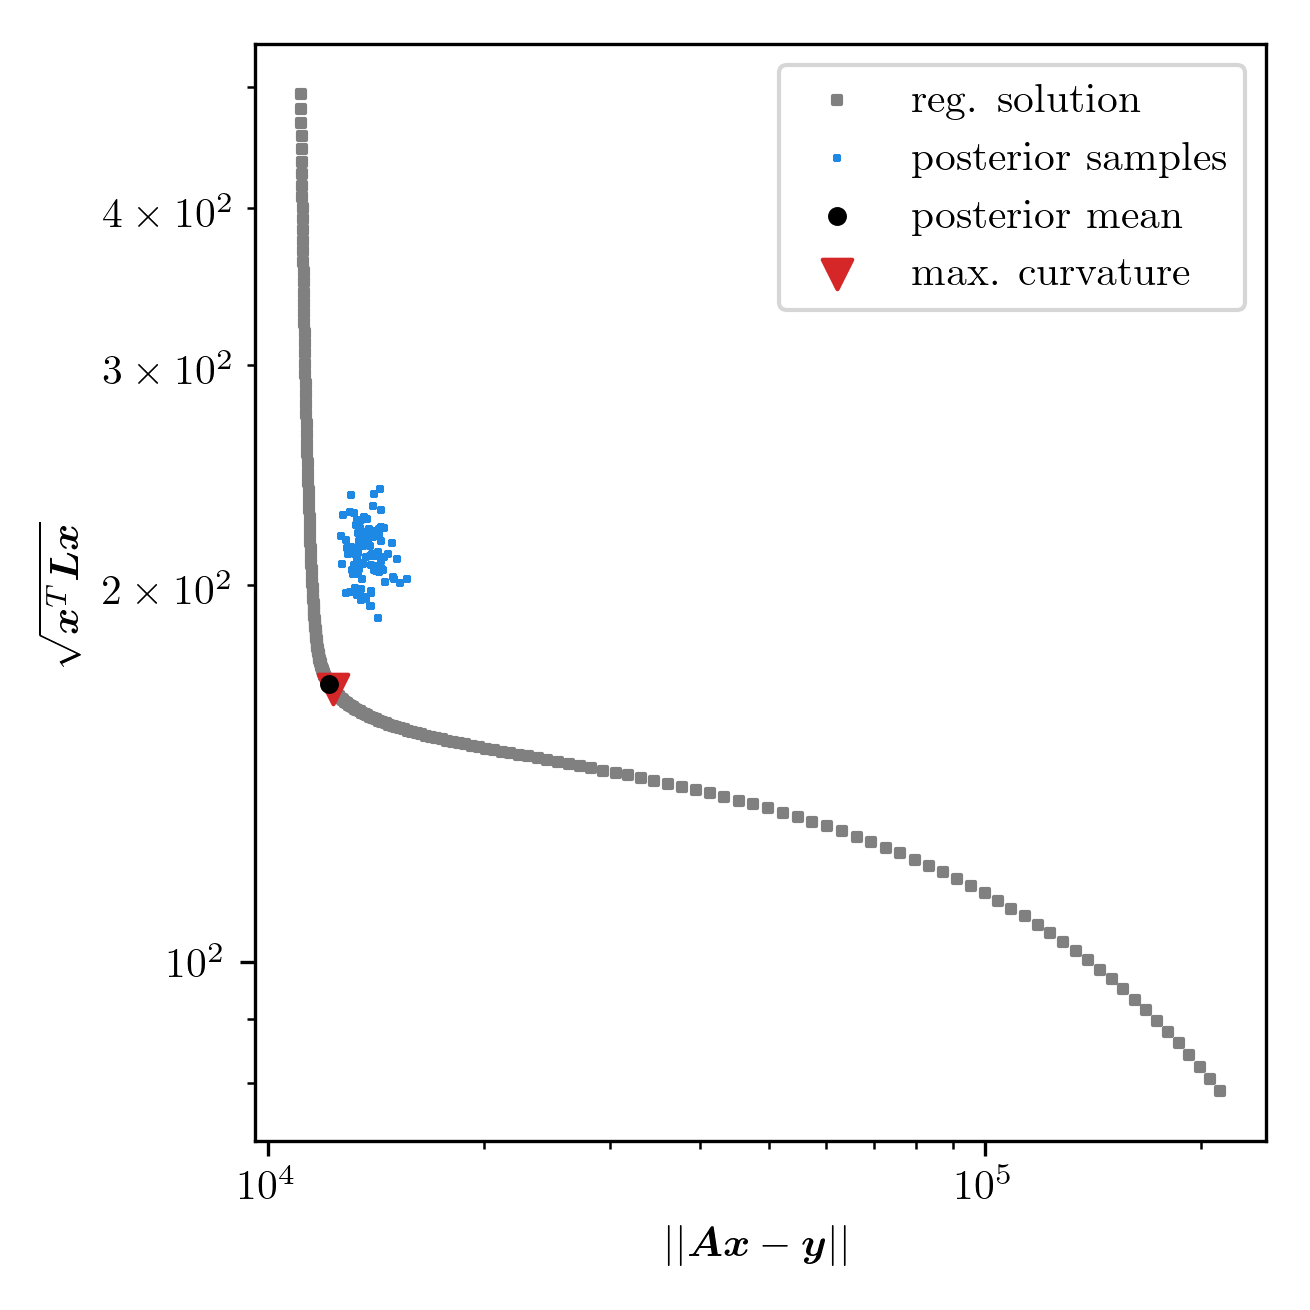
\includegraphics{LCurvePhD.png}
	\caption[Plot of the L-curve to find the regularised solution.]{We calculate regularised solution as in Eq. \ref{eq:} and plot the regularised semi norm $\sqrt{\bm{x}^T\bm{Lx}}$ against the data misfit norm $||\bm{Ax} -\bm{y} ||$ to find the regularised solution at the point of maximum curvature of the so-called L-Curve. Additionally we calculate the data misfit norm and the regularised norm for the ozone posterior and for samples of the conditional posterior distribution.}
	\label{fig:LCurve}
\end{figure}



\begin{figure}[ht!]
	\centering
	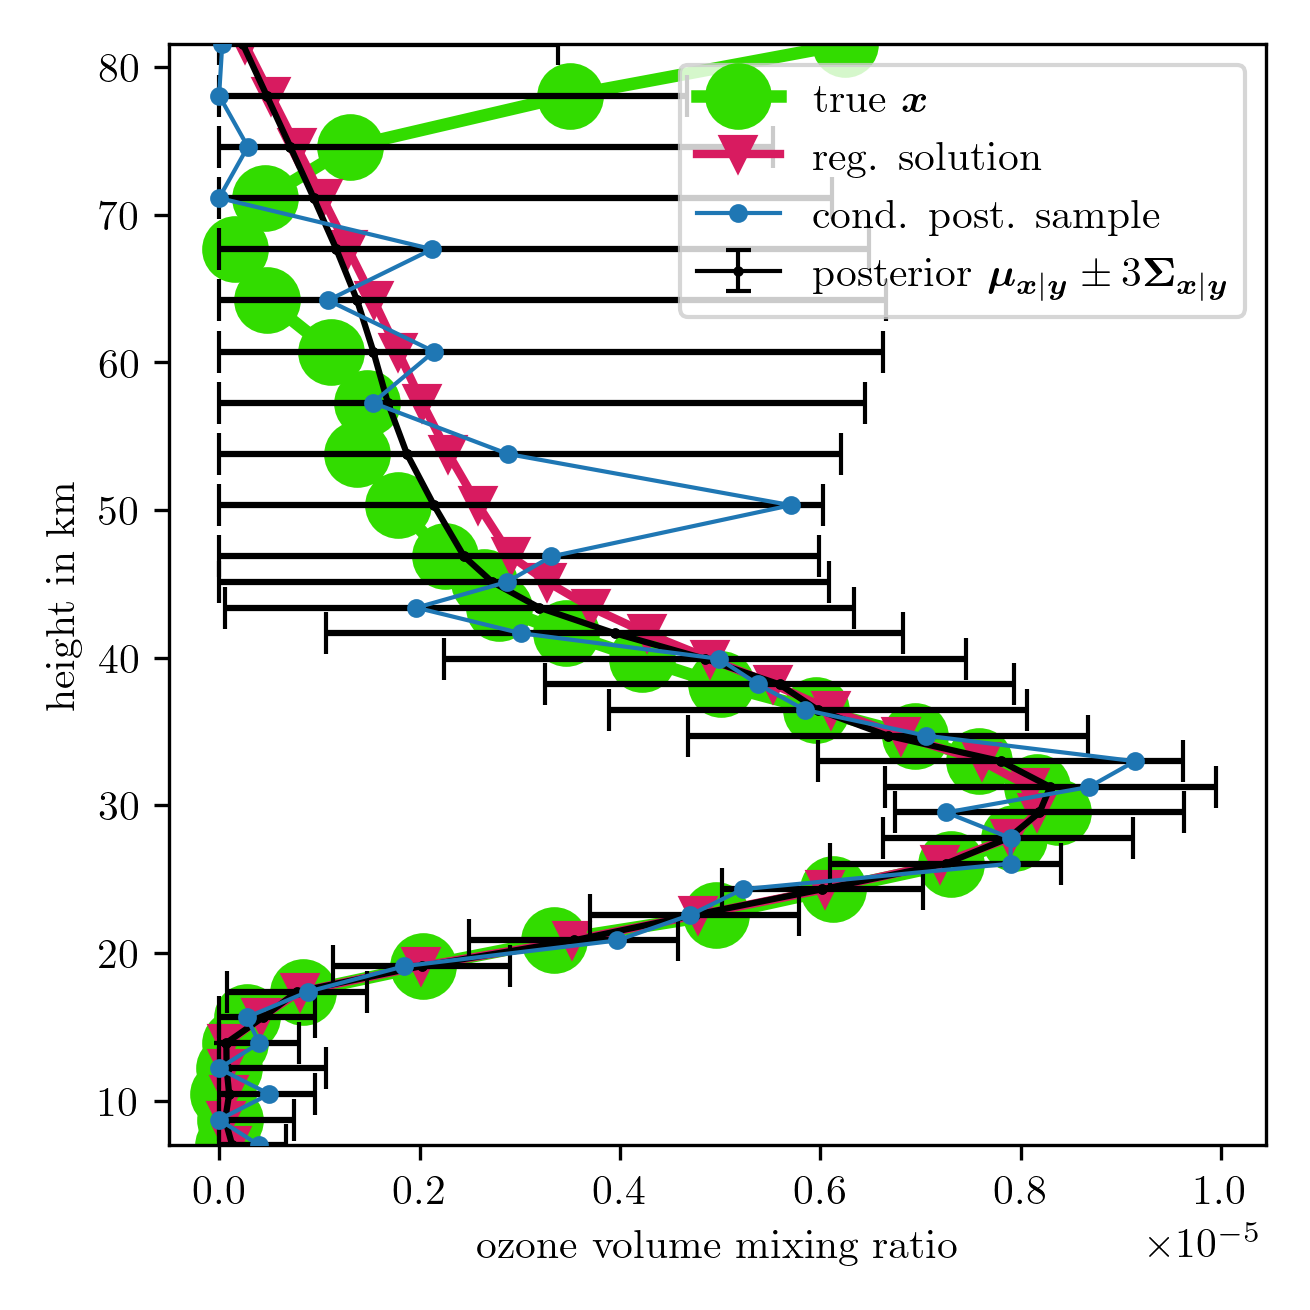
\includegraphics{SecRecResinclRegandSampl.png}
	%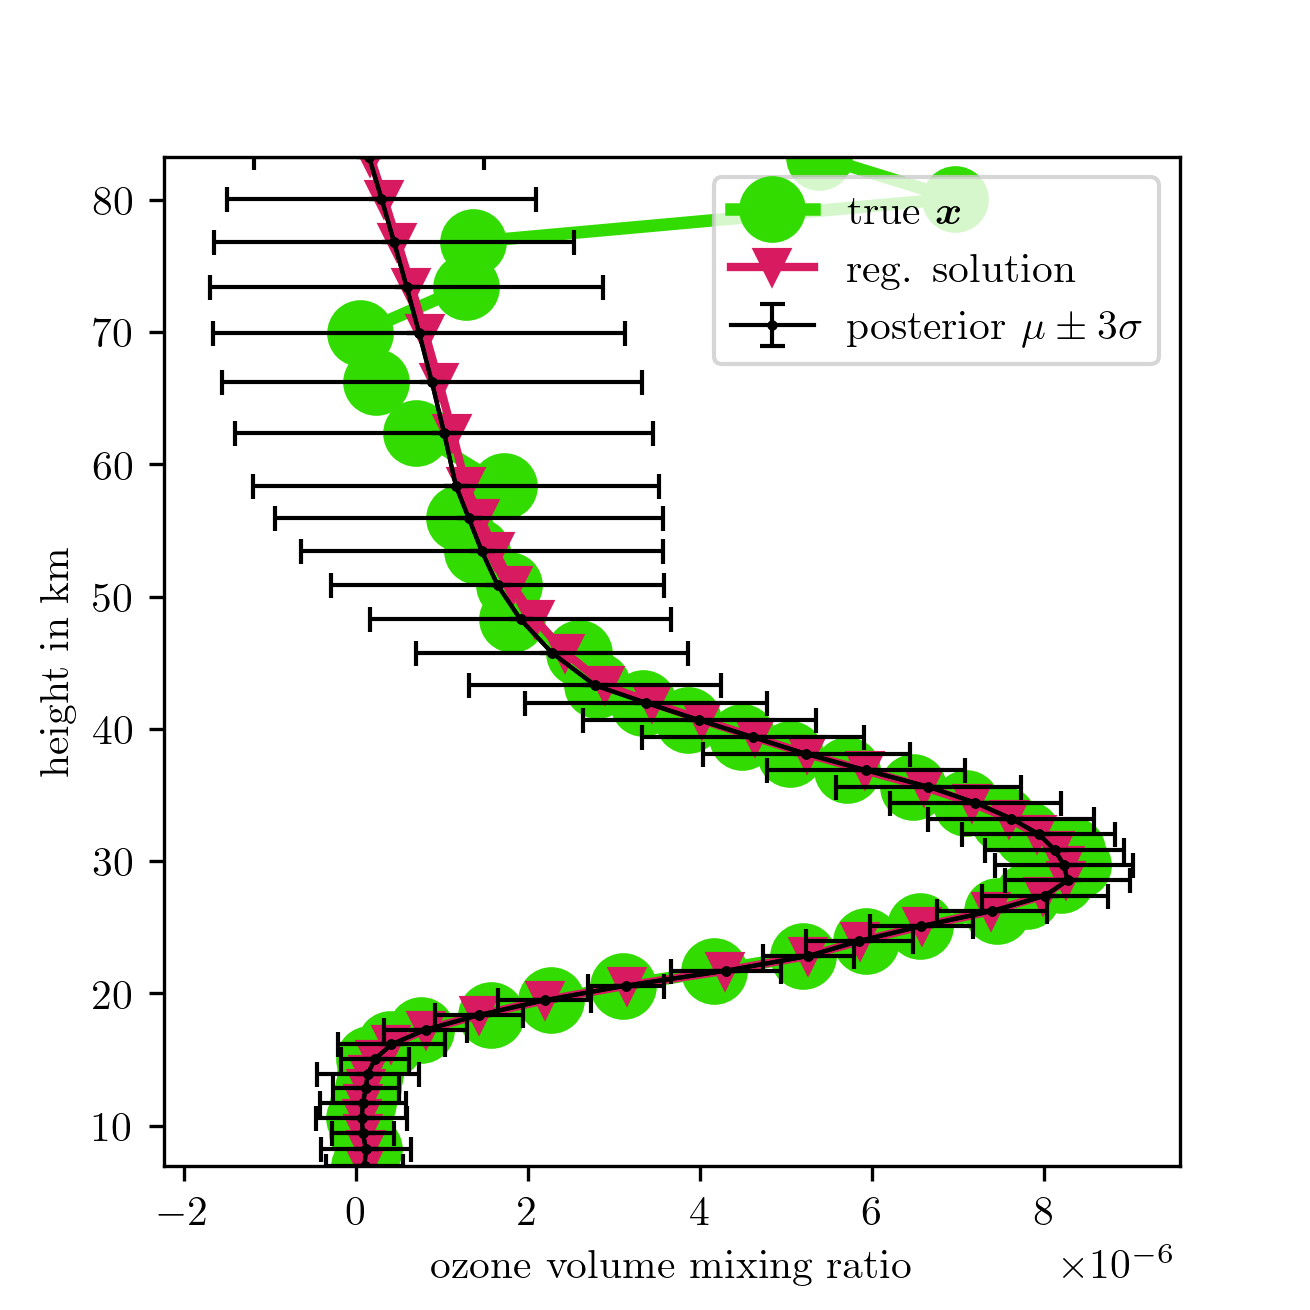
\includegraphics{SecRecResinclReg.png}
	\caption[Ozone posterior mean and variance and the regularised solution compared to the ground truth.]{We plot the conditional posterior mean and variance in black and the regularised solution on top of the ground truth ozone profile in green. We use the updated forward map $\bm{M}\bm{A}_L$}
	\label{fig:O3SolplsReg}
\end{figure}




\section{Posterior Pressure and Temperature}
\begin{itemize}
	\item make table with set up for TT and sampling t-walk
\end{itemize}
conditoned on an ozone smaple 
\begin{align*}
	\pi(h_1,p_0,b_1,b_2,\bm{h_T},\bm{c_T},\bm{a_T} | \bm{y}, \gamma, \bm{x}) &\propto \exp{\Bigl\{  -\frac{\gamma}{2} \left\Vert \bm{y}- \bm{A} \frac{\bm{p}}{\bm{T}}  \right\Vert_2^2 + \ln{\pi(h_1,p_0,b_1,b_2,\bm{h_T},\bm{c_T},\bm{a_T})} \Bigr\} } \\
	\pi(h_1,p_0,b_1,b_2,\bm{h_T},\bm{c_T},\bm{a_T} | \bm{y}) &\propto \pi(\bm{y}|h_1,p_0,b_1,b_2,\bm{h_T},\bm{c_T},\bm{a_T}) \pi(h_1,p_0,b_1,b_2,\bm{h_T},\bm{c_T},\bm{a_T}) \\
\end{align*}
TT set up
\begin{figure}[thb!]
	\centering
	\begin{tikzpicture}
		
		\node[align=center] at (-1,4) (A)    {$\bm{M A}_L$};
		\node[roundnode2] at (-1,2.5) (u)    {$\bm{u}$};
		\node[rectnode] at (-1,1) (y)    {$\bm{y}$};
		
		\node[roundnode2] at (3,6.5) (t)     {$\bm{T}$};
		\node[roundnode2] at (-1,6.5) (p)     {$\bm{p}$};
		\node[roundnode2] at (1,5) (pt)     {$\bm{p}/\bm{T}$};
		\node[roundnode2] at (0,8) (b1)    {$b$};
		%\node[roundnode2] at (1,8) (b2)    {$b_2$};
		\node[roundnode2] at (-2,8) (h1)    {$h_0$};
		\node[roundnode2] at (-1,8) (p0)    {$p_0$};
		\node[roundnode2] at (2.25,8) (ht)    {$\bm{h}$};
		\node[roundnode2] at (3.25,8) (ct)    {$T_0$};
		\node[roundnode2] at (4.25,8) (at)    {$\bm{a}$};
		
		%Lines
		\draw[->, very thick] (u.south) -- (y.north);
		\draw[->, mydotted, very thick] (A.south) -- (u.north);
		
		\draw[->, mydotted, very thick] (p.south east) -- (pt.north west);
		\draw[->, mydotted, very thick] (t.south west) -- (pt.north east);
		\draw[->, mydotted, very thick] (pt.south west) -- (A.east);
		\draw[->, mydotted, very thick] (h1.south) -- (p.north west);
		\draw[->, mydotted, very thick] (p0.south) -- (p.north);
		\draw[->, mydotted, very thick] (b1.south) -- (p.north east); 
		%\draw[->, very thick] (b2.south) -- (p.east); 
		
		\draw[->, mydotted, very thick] (ht.south) -- (t.north west);
		\draw[->, mydotted, very thick] (ct.south) -- (t.north);
		\draw[->, mydotted, very thick] (at.south) -- (t.north east);
		
		\node[align =center] at (-5,8) (T1) {posterior \\ over hyper-parameters \\ $\pi(h_0, p_0, b, \bm{h}, T_0, \bm{a}| \bm{y})$};
		
		\node[fit=(h1)(at),draw,dotted,black, rounded corners] {};
	\end{tikzpicture} 
\caption[Directed acyclic Graph for pressure and temperature.]{Conditioned on an ozone profile the posterior of the hyper-parameters describing pressure and temperature is given as in Eq. \ref{eq:}. Since pressure and temperature go into the forward model as $\bm{p}/\bm{T}$ they are highly correlated but the pressure is the dominant parameter, see Fig. 
	\ref{fig:PriorPressOverTemp} and \ref{fig:SeaLevelHist}. Note that here we use the updated forward model $\bm{M} \bm{A}_L$ and conditioned on a $\gamma$ sample from the previously evaluated marginal posterior see Fig. \ref{fig:MargPostHistTT}. }
	\label{fig:DAGPT}
\end{figure}

\begin{figure}[ht!]
	\centering
	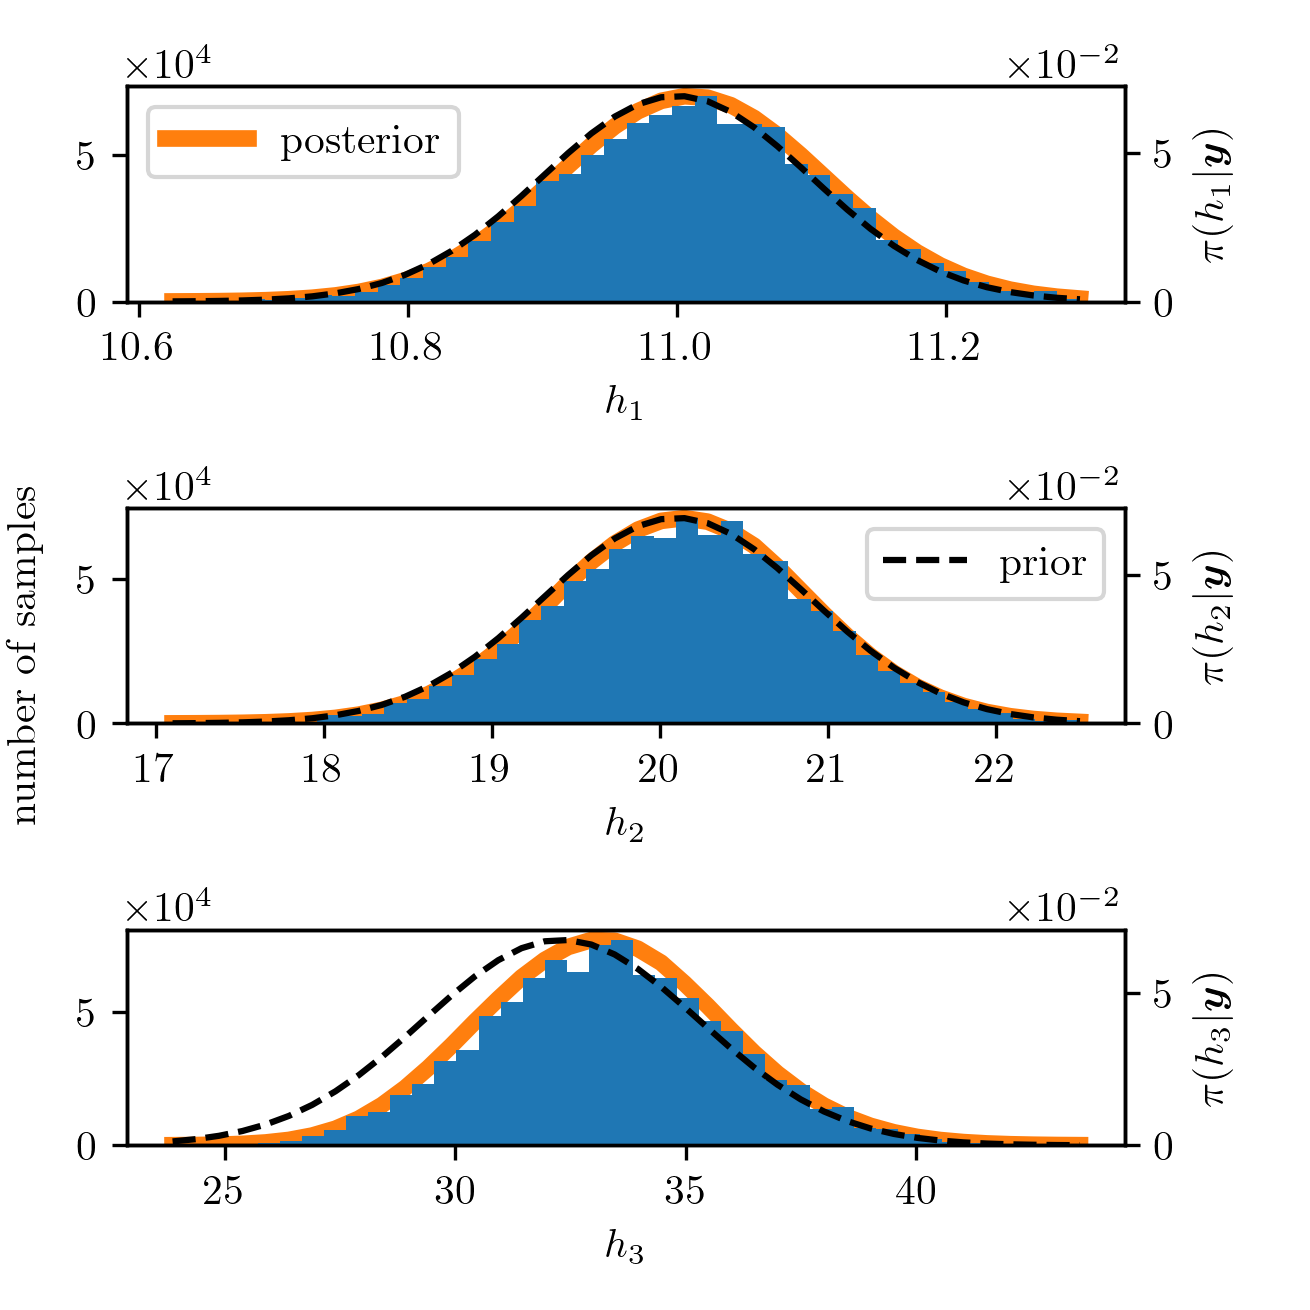
\includegraphics{PHdPTPost0.png}
	\caption[Histograms and TT approximation of posterior distribution as well as hyper-prior distribution.]{We plot the TT approximation of marginal posterior in orange and the samples as a histogram as well as the prior distribution with a dotted line.}
	\label{fig:PostHistTT0}
\end{figure}
\begin{figure}[ht!]
	\centering
	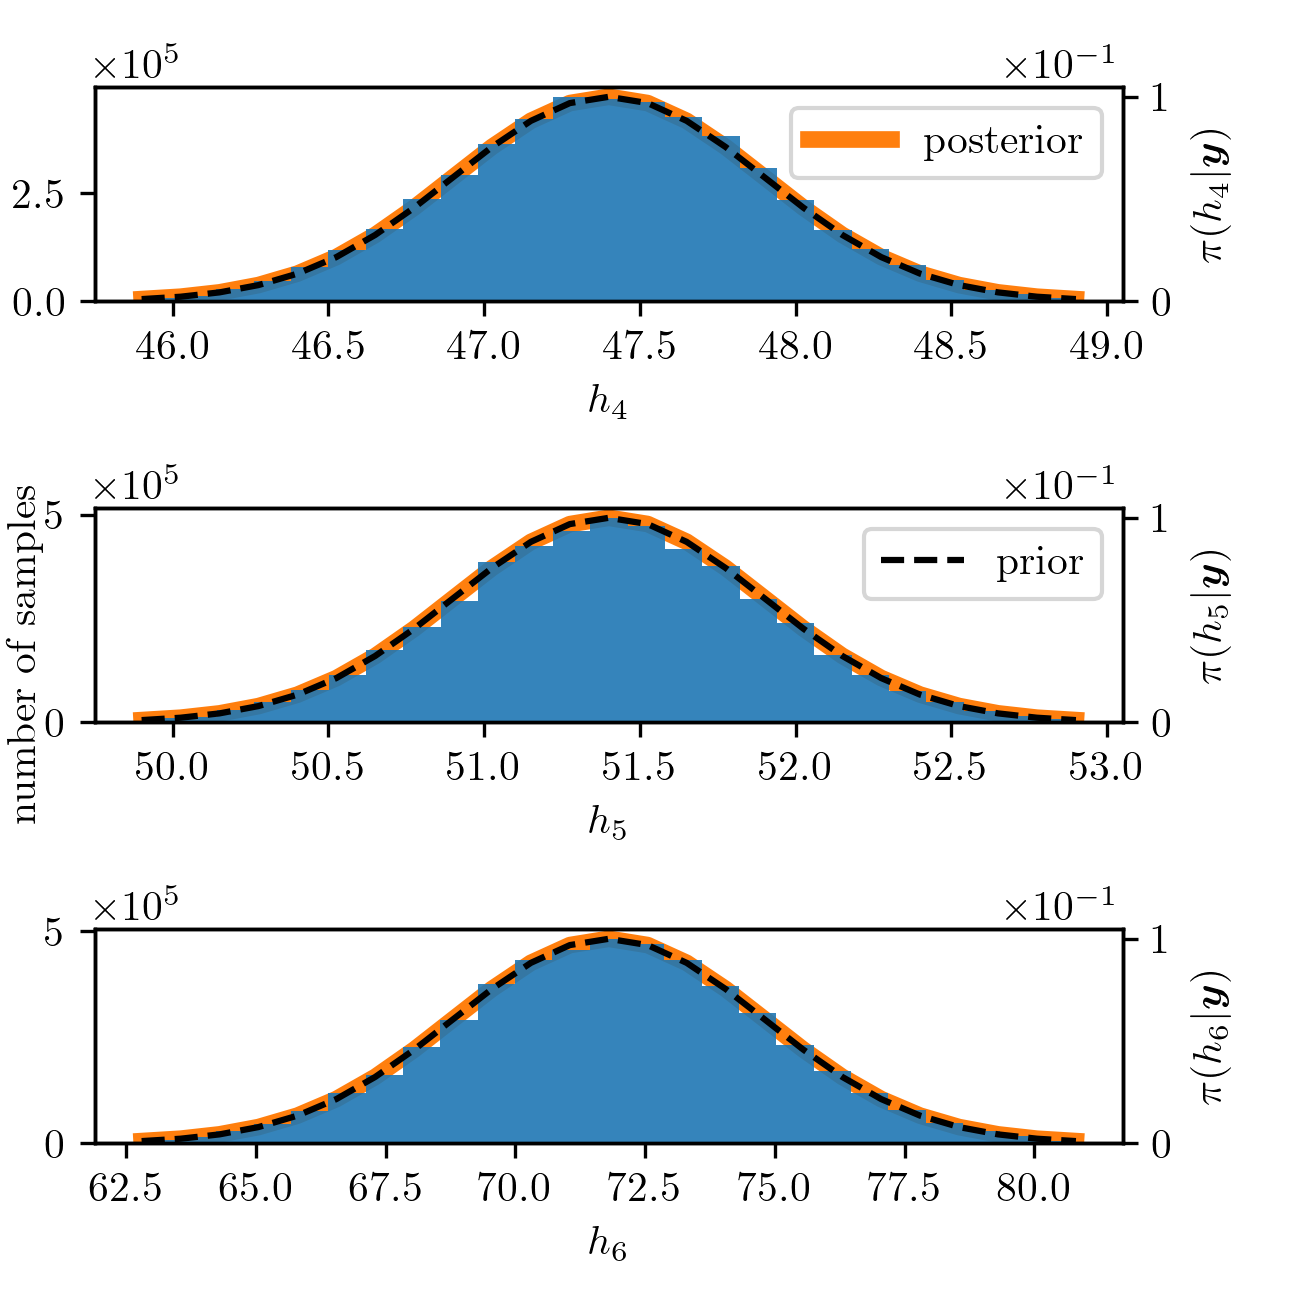
\includegraphics{PHdPTPost1.png}
	\caption[Histograms and TT approximation of posterior distribution as well as hyper-prior distribution.]{We plot the TT approximation of marginal posterior in orange and the samples as a histogram as well as the prior distribution with a dotted line.}
	\label{fig:PostHistTT1}
\end{figure}
\begin{figure}[ht!]
	\centering
	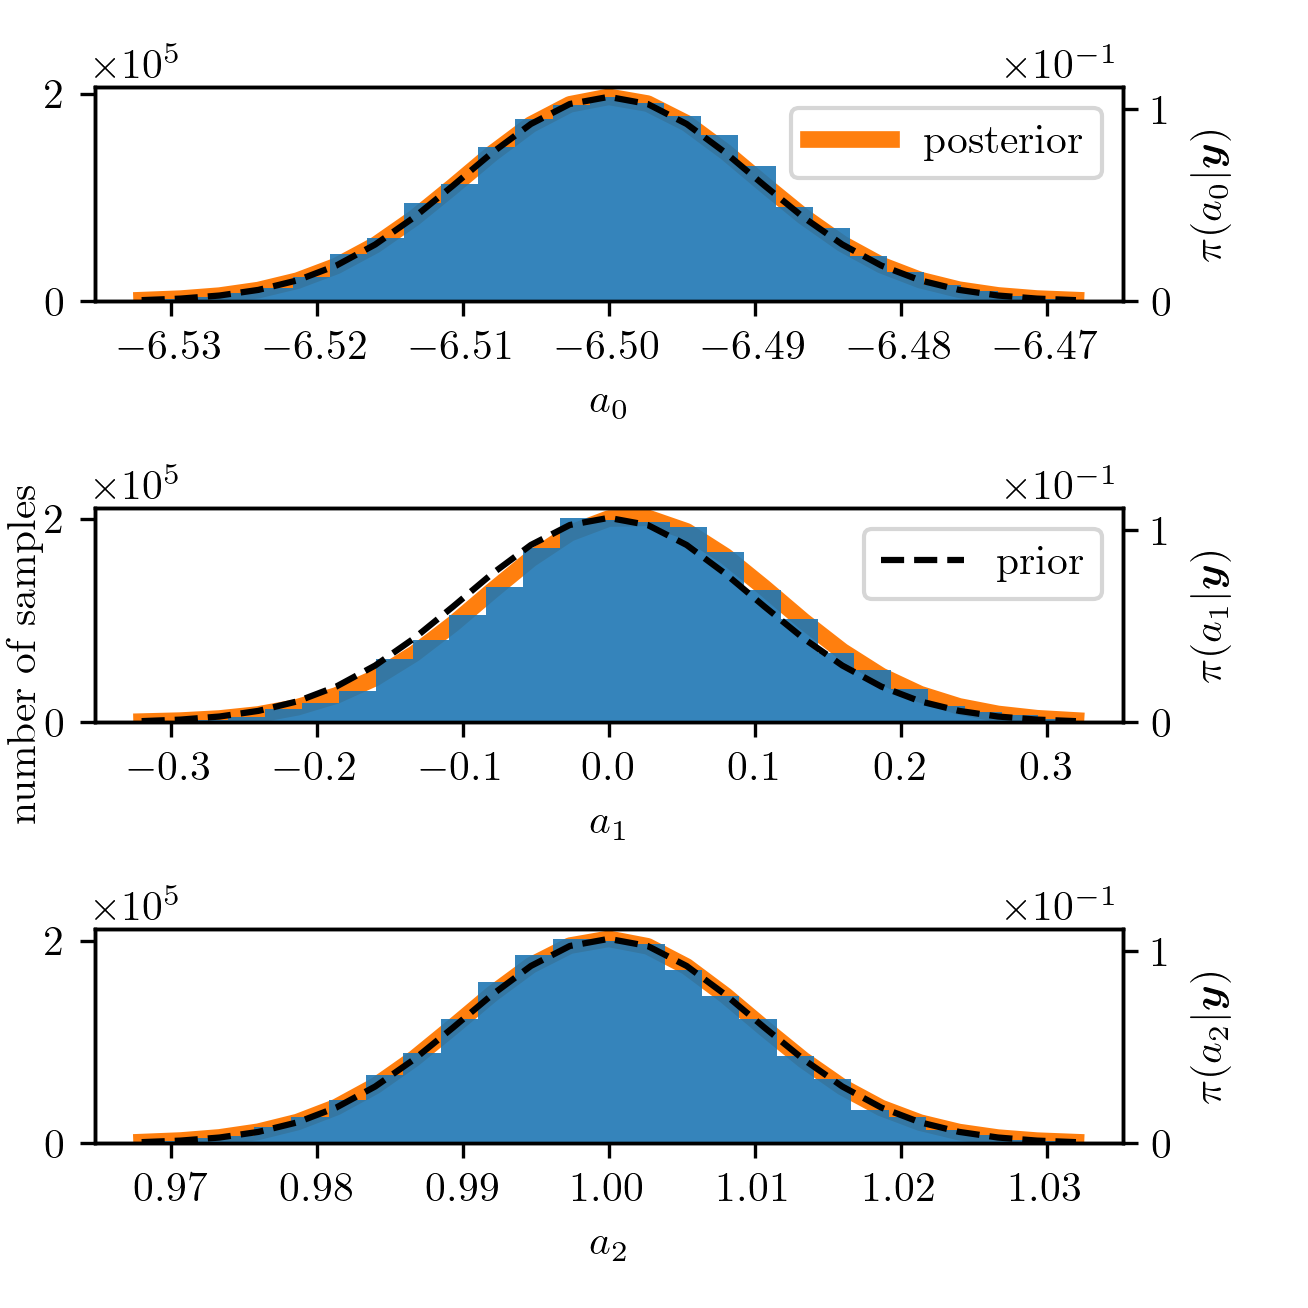
\includegraphics{PHdPTPost2.png}
	\caption[Histograms and TT approximation of posterior distribution as well as hyper-prior distribution.]{We plot the TT approximation of marginal posterior in orange and the samples as a histogram as well as the prior distribution with a dotted line.}
	\label{fig:PostHistTT2}
\end{figure}
\begin{figure}[ht!]
	\centering
	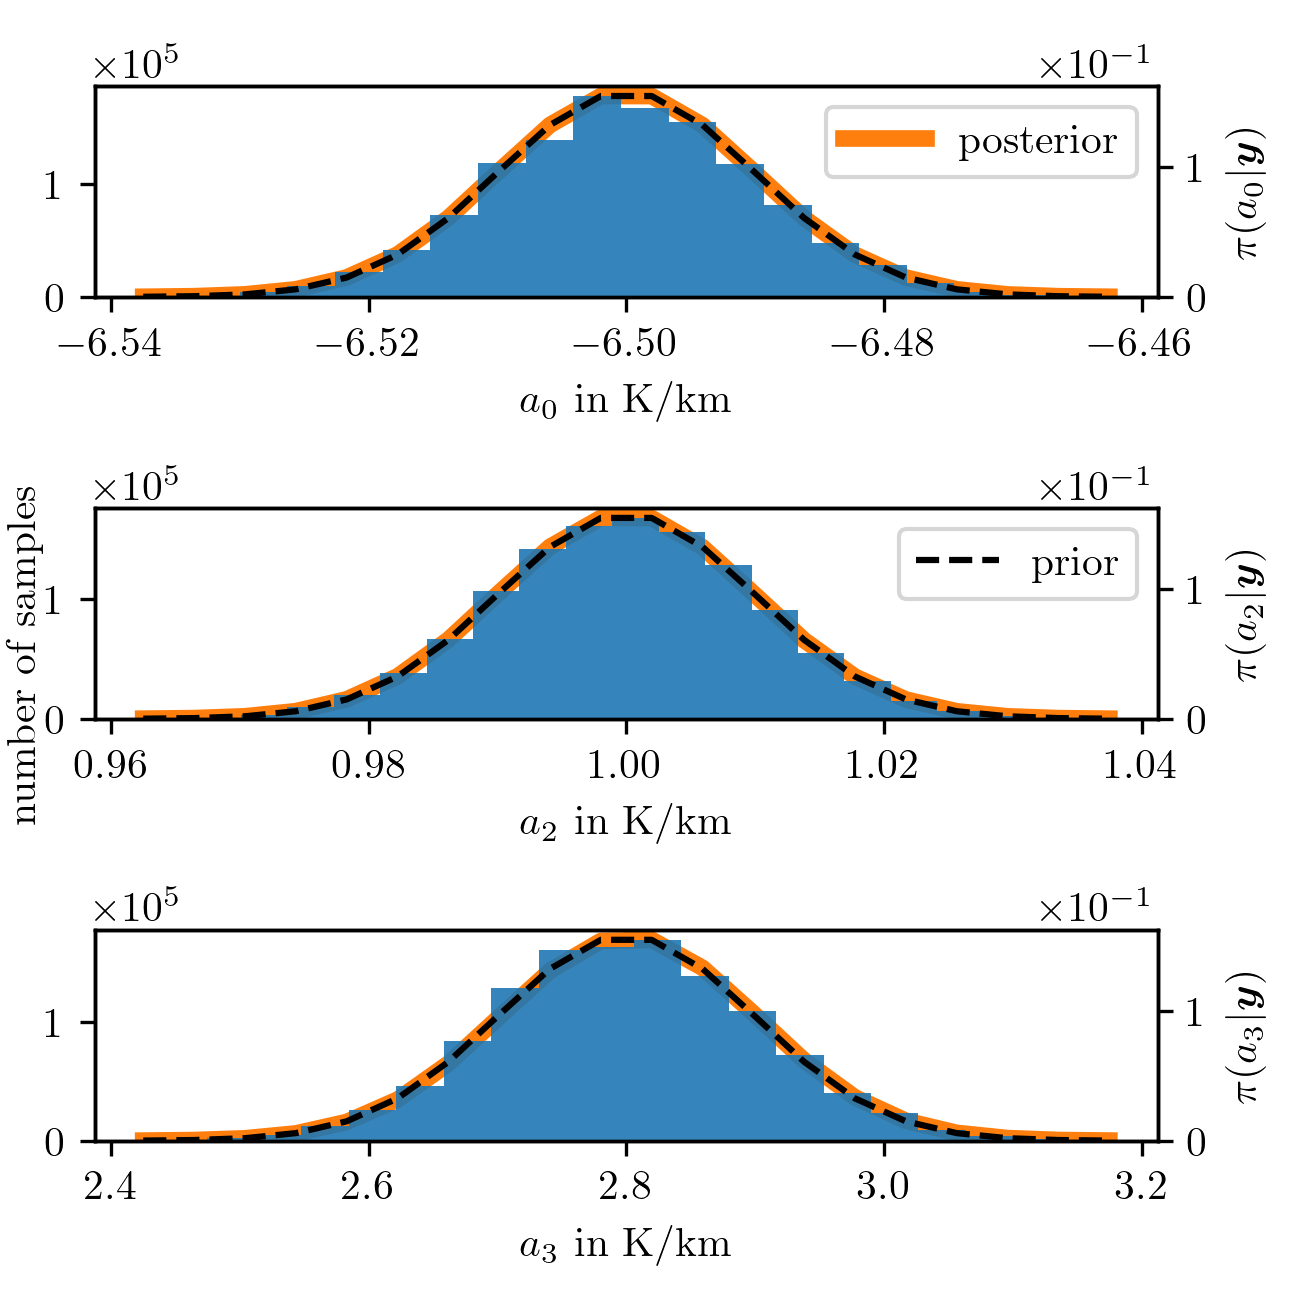
\includegraphics{PHdPTPost3.png}
	\caption[Histograms and TT approximation of posterior distribution as well as hyper-prior distribution.]{We plot the TT approximation of marginal posterior in orange and the samples as a histogram as well as the prior distribution with a dotted line.}
	\label{fig:PostHistTT3}
\end{figure}
\begin{figure}[ht!]
	\centering
	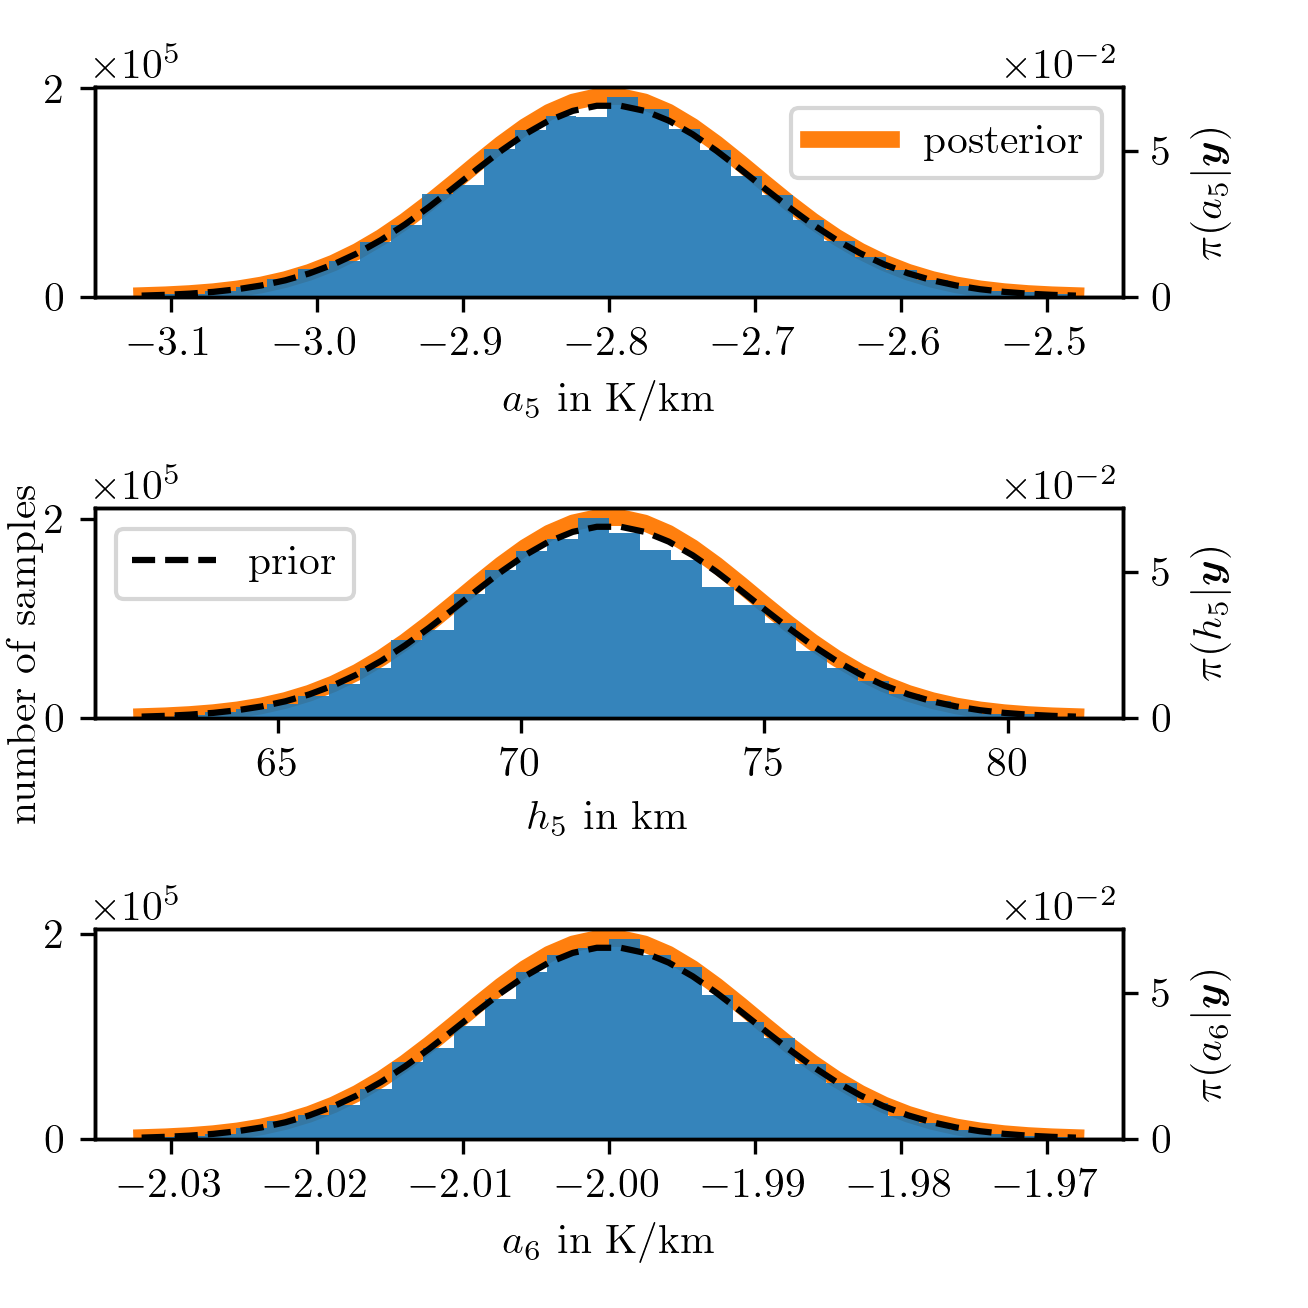
\includegraphics{PHdPTPost4.png}
	\caption[Histograms and TT approximation of posterior distribution as well as hyper-prior distribution.]{We plot the TT approximation of marginal posterior in orange and the samples as a histogram as well as the prior distribution with a dotted line.}
	\label{fig:PostHistTT4}
\end{figure}

\begin{figure}[ht!]
	\centering
	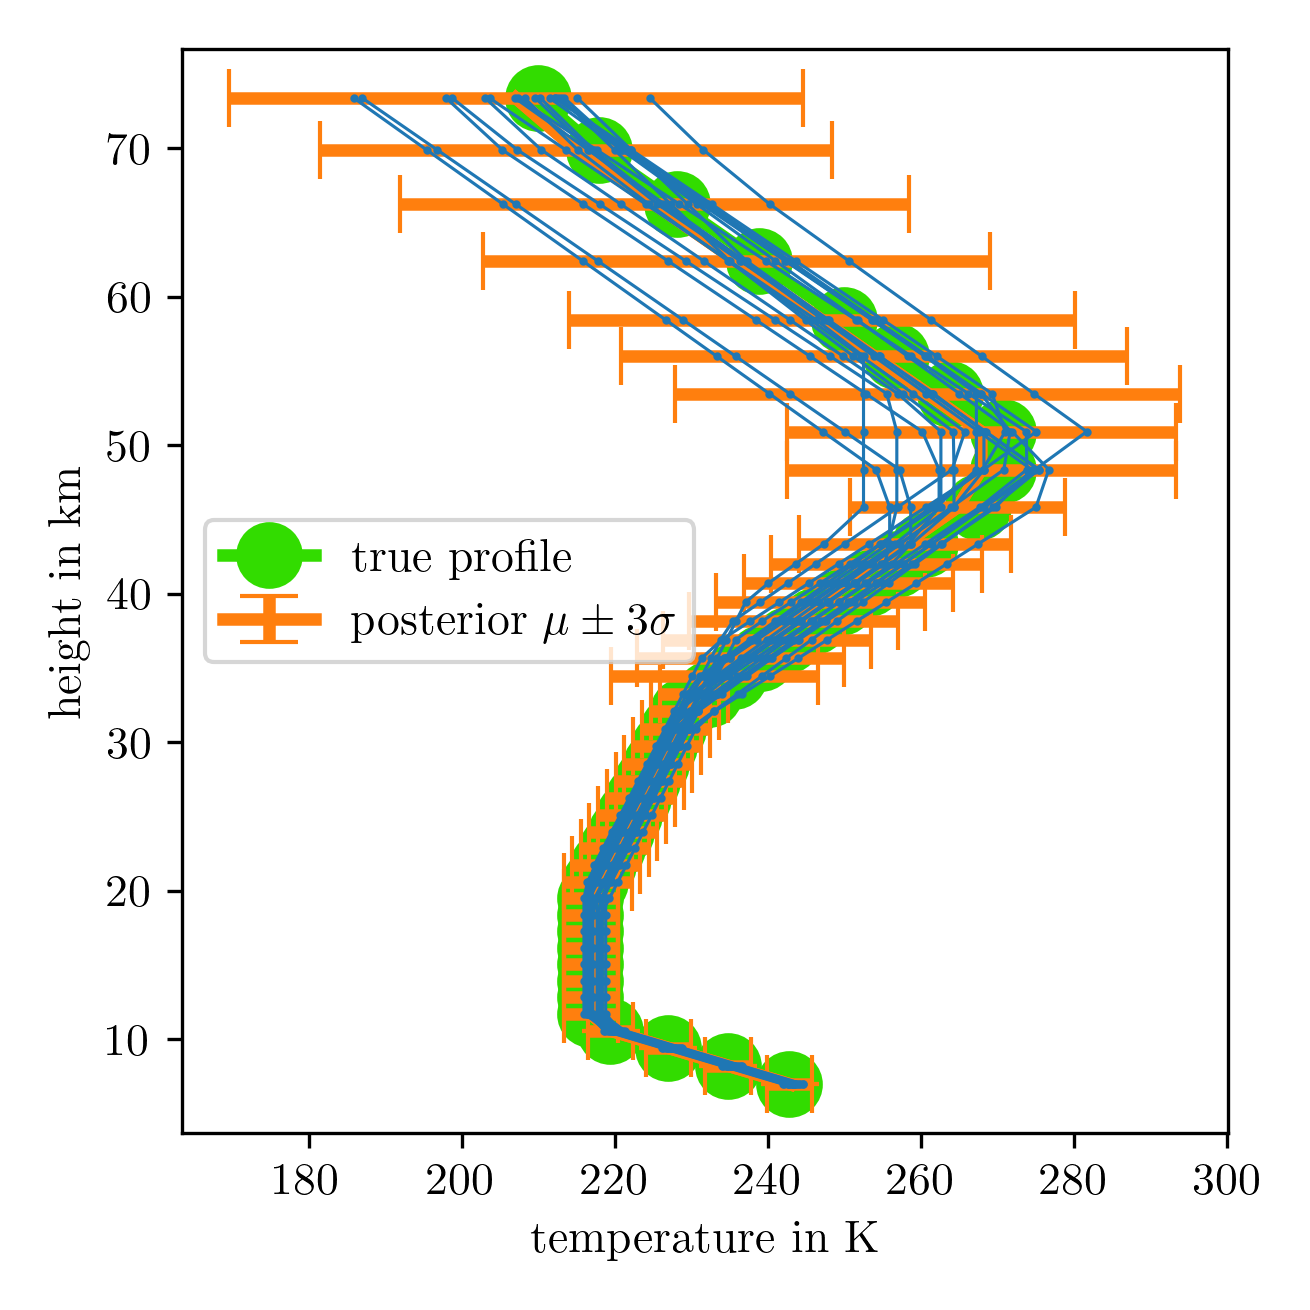
\includegraphics{TempPostMeanSigm.png}
	\caption[Temperature posterior samples.]{We take samples from the posterior distribution, as plotted in Figures \ref{fig:PostHistTT0} to \ref{fig:PostHistTT3} and plot the corresponding temperature function, see Eq: \ref{eq:tempFunc}. }
	\label{fig:TempPost}
\end{figure}

\begin{figure}[ht!]
	\centering
	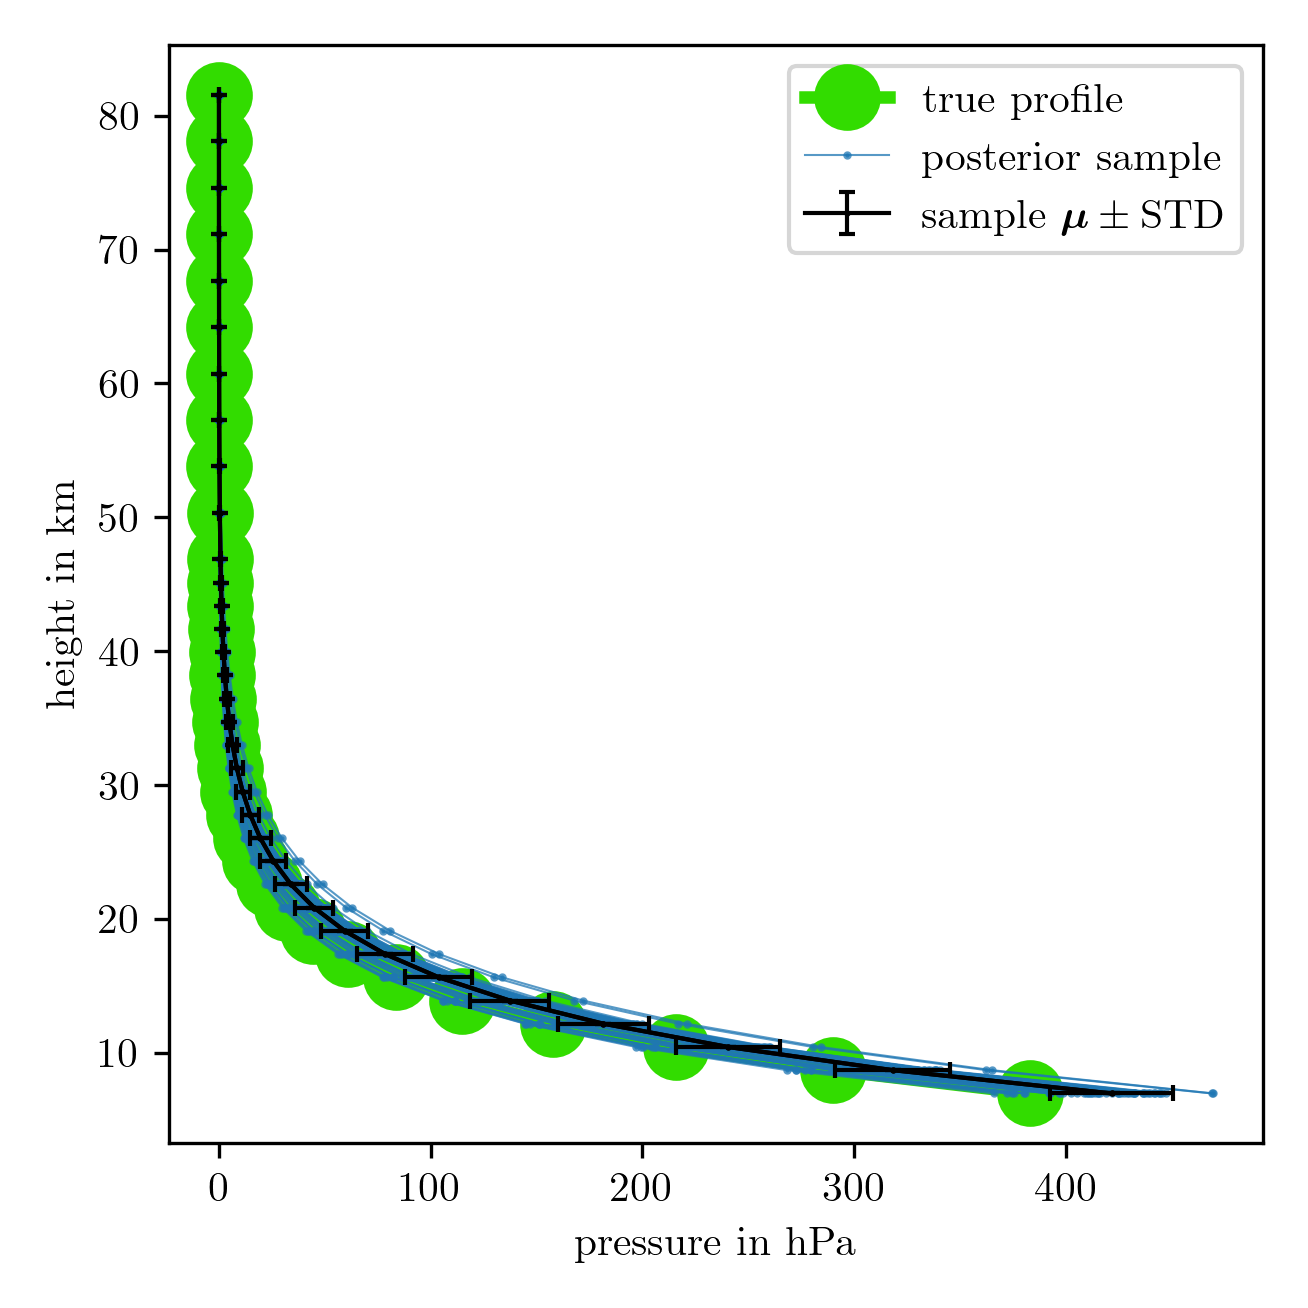
\includegraphics{PressPostMeanSigm.png}
	\caption[Pressure posterior samples.]{We take samples from the posterior distribution, as plotted in Fig. \ref{fig:PostHistTT4} and plot the corresponding pressure function, see Eq: \ref{eq:pressFunc}.}
	\label{fig:PressPost}
\end{figure}



%@misc{MLSdata,
%	title= {MLS/Aura Level 2 Ozone (O3) Mixing Ratio V005},
%	author = {Schwartz, M., Froidevaux, L., Livesey, N. and Read, W.},
%	year = {2020},
%	howpublished ={\url{https://disc.gsfc.nasa.gov/datasets/ML2O3_005/summary?keywords=mls%20o3}},
%	publisher = {Goddard Earth Sciences Data and Information Services Center (GES DISC)},
%	adress = {Greenbelt, MD, USA},
%	note = "[Online; accessed 25/04/24, 10.5067/Aura/MLS/DATA2516]"
%}


